% !TEX TS-program = pdflatex
% !TEX encoding = UTF-8 Unicode

\documentclass[12pt]{report} % use larger type; default would be 10pt

\usepackage[utf8]{inputenc} % set input encoding
\usepackage{mystyle}



\title{Master Thesis \\
\bf{Swarm of autonomous MAVs in urban Search and Rescue applications} }
\author{Francesco Wanderlingh}
\date{September, 2014}

\DeclareRobustCommand{\SkipTolEntry}[5]{}
\graphicspath{{img/}}
\newcommand{\HRule}{\rule{\linewidth}{0.4mm}} % Change HRule default width
\providecommand{\e}[1]{\ensuremath{\times 10^{#1}}} % Exponential notation

%%% The "real" document content comes below...

\begin{document}


\nocite{*} %Include articles in bibliography even if they are not cited.


\begin{titlepage}

% Marcelo de Faria Version
%\begin{frame}
%
%\begin{picture}(18,1)
%\put(-36,-67.5){\includegraphics[scale=0.85]{wut_logo}}
%\put(400.5,-70.5){\includegraphics[scale=0.25]{mel_logo}}
%\end{picture}
%
%\LARGE  {\bf{\hspace{1.2cm} Warsaw University of Technology}} 
%\vskip 0.2 cm
%\hspace{1.3cm} \large {\bf{Faculty of Power and Aeronautical Engineering}}
% \vskip 0.3 cm
%\hspace{2.0cm} { {\large {Division of Theory of Machines and Robots}}}
%
%\end{frame}


\begin{center}

% My Version - more centered
\begin{table}[ht]
\centering
\begin{adjustbox}{right=15.3cm}
\begin{tabular}{c >{\centering}m{12cm} c}
\raisebox{-.45\height}{\includegraphics[scale=0.85]{wut_logo}} &
\Large {\textbf{Warsaw University of Technology}} 
\vskip 0.2 cm
\large {\textbf{Faculty of Power and Aeronautical Engineering}}
\vskip 0.3 cm
{ {\large {Division of Theory of Machines and Robots}}} &
\ \ \ \raisebox{-.45\height}{\includegraphics[scale=0.25]{mel_logo}}
\end{tabular}
\end{adjustbox}
\end{table}

\hrule

\vskip 1cm

\Large{Diploma Thesis} \\ 
\large Master Degree

\vskip 1.5 cm

\large{Francesco \textsc{Wanderlingh}}

\vskip 1 cm 

\Large{\textbf{Swarm of autonomous MAVs in urban Search and Rescue applications}}

\normalsize
\vskip 2 cm
\hfill Student ID: 263870 \\
\hfill Robotics and Automation  \\ 
\hfill European Master on Advanced Robotics (EMARO)

\begin{flushleft}
\vskip 2 cm
\textbf{Supervisor: }{\large Prof. Wojciech \textsc{Szynkiewicz} - WUT Poland} \\
\textbf{Co-Supervisor: }{\large Prof. Antonio \textsc{Sgorbissa} - UNIGE Italy} \\
\textbf{Co-Supervisor: }{\large Prof. Cristiano \textsc{Nattero} - UNIGE Italy}
\end{flushleft}

\vfill


% Bottom of the page
{\large Warsaw, September 2014}
\end{center}
\end{titlepage}


\pagenumbering{gobble}
\null\newpage


\input{./tex/0.1_Authors_Declaration}
\null\newpage
\begin{center}
\Large {\textbf{Swarm of autonomous MAVs in Urban Search and Rescue applications}}\\
\large {by  \\
Francesco Wanderlingh}
\end{center}

\vskip 1cm
\Large {\textbf{Abstract}} \\ 

\large{
In the framework of swarm robotics involved in search and rescue applications, the main purpose of this thesis is to investigate complete 
terrain coverage algorithms. These kinds of algorithms are intended in the first place to perform a fast monitoring by means of aerial 
imaging, but many other applications are possible. Two main classes can be identified in the algorithms developed for the terrain coverage: 
online and offline coverage methods. For the online class the algorithms taken into account are Node Counting, Learning Real-Time A*, Edge 
Counting and PatrolGRAPH*. For the offline class instead the coverage problem was formulated as a Vehicle Routing Problem and solved with a 
greedy approach. In a first phase the algorithms were tested in a 3D simulation environment and a large number of results was collected and 
compared. Finally the whole framework was tested performing the coverage using real multi-copters. }
\clearpage
\null\newpage

\begin{center}
\Large {\bf{Zastosowania roju autonomicznych miniaturowych statków powietrznych w poszukiwaniu i ratownictwie miejskim}}\\
\large {przez  \\
Francesco Wanderlingh}
\end{center}

\vskip 1cm
\Large {\textbf{Streszczenie}} \\


\large{
Głównym celem pracy jest analiza algorytmów całkowitego pokrycia terenu z~użyciem roju miniaturowych statków powietrznych 
w~poszukiwaniu i ratownictwie miejskim. Algorytmy te są przeznaczone, przede wszystkim, do szybkiego monitorowania terenu 
z~użyciem obrazowania z~powietrza, aczkolwiek możliwych jest wiele innych zastosowań. Wyróżnia się dwie główne klasy algorytmów 
przeszukania terenu: metody \emph{on-line} i \emph{off-line}. Do pierwszej z nich można zaliczyć algorytmy: Node Counting, 
Learning Real-Time A*, Edge Counting and PatrolGRAPH*. W~podejściu \emph{off-line} zadanie pokrycia terenu zostało sformułowane 
jako problem marszrutyzacji i rozwiązano go za pomocą algorytmów zachłannych przeszukiwania grafu. W pierwszej fazie badań algorytmy 
były testowane w~symulacji w~stworzonym środowisku 3D. Wykonano wiele testów, a ich wyniki zostały zebrane i porównane. Następnie przeprowadzono 
eksperymenty pokrycia terenu z~użyciem rzeczywistych multikopterów.   
}
\clearpage

\null\newpage

\normalsize % Needed since the introduction of the abstract file was unexpectedly messing everything up

\pagenumbering{roman}
\tableofcontents
\listoffigures
\listoftables

\clearpage

\onehalfspace
\pagenumbering{arabic}

\chapter{Introduction}

\section{General motivation and objectives}

When natural disaster occur, a prompt intervention is a key factor. In order to organize effective rescue missions, it is fundamental to quickly gather information about collapsed buildings, damaged roads and, above all, victims. To this extent, autonomous Micro Aerial Vehicles (MAVs) are a promising technology to survey the stricken area.

The introduction of unmanned aerial vehicles (UAVs) has revolutionized military operations all over the world. In the past year, the U.S. reached an important milestone in that Air Force now has more UAVs than manned aircraft, while Israel and the United Kingdom had recent significant advances in UAV heavy-lift capacity \cite{6099676}. These advances are not only limited to the military as the international civil sector also looks to such unmanned technologies to aid operations such as fighting forest fires, undersea exploration, monitoring wildlife, inspecting bridges, and supporting first responders such as police and rescue organizations. UAV expenditures alone are predicted to more than double in the next ten years, and are expected to exceed \$80 billion \cite{6099676}.
So far this century there have been more than 1000 fatal earthquakes causing a total loss of life exceeding 1.5 million people. Reducing the loss of life is the primary priority of most earthquake protection strategies, and yet the processes that contribute to death tolls and the best strategies for reducing injury levels are not well understood. According to \cite{coburn1994death}, structural collapses are responsible for 75\% of deaths in earthquakes. The factors influencing the number of victims per building collapse fall into five major categories M1 to M5. Being M3 the “occupants trapped by collapse”.

In all three cases it’s evident how a flying vehicle can be useful to reach the areas struck by the earthquake. When disasters such as this occur, a prompt intervention is a key factor: the probability of saving lives decreases dramatically after the initial hours. In order to organize effective rescue missions, it is fundamental to quickly gather information about collapsed buildings, damaged roads and, above all, victims. To this extent, autonomous Micro Aerial Vehicles (MAV) are a promising technology to survey the stricken area. 
These applications usually require complete autonomy in navigation, small size of the air vehicle to access also confined out and indoor spaces and low power consumption for extended operation times. 


In the framework of swarm robotics involved in search and rescue (SAR or S\&R) applications, the main purpose of this thesis research is to investigate complete coverage algorithms. These kind of algorithms are intended in the first place to perform a fast monitoring by means of aerial imaging, but many other applications are possible.

The branch of swarm robotics is relatively new, and the application of swarm robotics to flying vehicles is even more innovative. The capacity of having multiple robots with such mobility in fact opens new possibilities with respect to terrain exploration.

I developed in parallel two different approaches: real-time and optimised coverage. They fit different hardware and swarm-type requirements, but they share the same mathematical base, graph theory.

To test the algorithms a 3D simulation environment was created and the simulated robots are controlled using the ROS robotic platform. This was mandatory choice for testing online algorithms, but nevertheless a good way to visualise the results for pre-processed optimised coverage.
The simulated environment has been represented as a graph using a convention shown in the next chapter, on which the algorithms operate to perform the coverage. As a last step the algorithms were also tested with success on a pair of real multi-copters available in the laboratory, proving that a consistent framework is available for immediate application.


\section{The Coverage Problem}

This thesis work deals with the problem of finding the most effective algorithm to solve the coverage problem. Let's then start defining what the coverage problem deals with and how we can solve it.

 The are two major classes in which we can divide coverage problems: \emph{static} coverage and \emph{dynamic} coverage. Given a finite area with obstacles to cover, the static coverage solves the problem of finding the best robot positions such that visibility of the area is maximized. In this case then there will be some which will not be monitored by the robots (blind spots) and for our SAR purposes this is unacceptable. For this reason in the thesis we opted for a dynamic approach to coverage. In a dynamic coverage the robot will have to cover the area by exploring it thoroughly, so even if at each time step we just observe a little portion of the terrain, the final knowledge of the area is complete. If for example we have to find a victim in a stricken environment and the person is hidden in a blind spot, the static coverage does not ensures that the victim will be detected, while the dynamic coverage does. A static coverage moreover does not observe the area uniformly; the regions near to the robot will be well monitored while far one will be observed only marginally.
 
Now in the the field of dynamic coverage we can identify two classes:
\begin{itemize}
\item \textbf{Offline coverage}: the paths are pre-calculated with a routing algorithm, before the robot start exploring the environment
\item \textbf{Online coverage}: the robots decide their path while they are exploring the environment, by making decisions based on the current knowledge they have on the coverage completion
\end{itemize}

An important aspect to take into account is whether the coverage is meant to be performed by a single robot, or by a group of robots. The main difference between the two is that in the single robot the robot does not have to interact with other moving units and this simplifies the planning and does not require a inter-robot communication system. In the multi-robot coverage instead the communication between units is essential to take advantage of a collaborative behaviour. In this thesis the main objective has been to build a flexible software framework that can  be easily extend from a single-robot to multi-robot configuration seamlessly.

For known environments it is important to accomplish the coverage task in the minimum possible time and using this a priori knowledge we can construct an algorithm that computes the optimal paths to completely cover the area. This is possible decomposing the environment in a finite number of spots to visit (see next section, \ref{sec:spaceDec}) and by modelling the coverage as a routing problem where we have to visit all the location at least once. But due to the huge size of the solution space, using offline algorithms to find optimal path turns out to be not so trivial, optimal solution are really hard to compute, actually NP-hard \cite{wiki:VRP}, so in practice heuristic and deterministic methods have been developed that find acceptably good solutions for the VRP. This involves a discrete computation capability and in the perspective of using the algorithms to guide autonomous robots this can represent a limitation. That is why several online strategies have also been investigated.
From a computational point of view online algorithms are far less challenging. In an online coverage basically, every time the robot reaches a certain position on the map, it has the only simple task of choosing what point to reach next basing its decision only the local knowledge it has on the map (\emph{local} with respect to its position in space). It also has the advantage of being more flexible; think of a situation where a robot fails due to a crash: in an offline coverage the path are pre-calculated so the path assigned to that robot will not be covered, in an online case instead the robots will continue exploring the area till they know that the whole area is covered. They also fit better the swarm robotics approach where complex behaviours emerge from the sum of many simple ones.

As a final remark since performing SLAM (simultaneous localization and mapping) is out of the scope of this thesis the terrain is assumed to be known. Having in mind that by using any modern web mapping service the topology of the area can be retrieved this can be a reasonable assumption in real world applications.

The path planning required to perform the complete coverage task must be build on top of an abstract representation of the terrain. This abstract representation can be obtained through one of the various methods discussed in the next section.



\section{State of the art}

Many works have been present in the area of research dealing with the coverage problem, either offline or online, aiming to accomplish static or dynamic coverage, using single or multi-robot approach, and assuming known and unknown environments. In this paragraph we will review some of the solutions found in literature as a starting point for the research developed in this thesis.


\subsection{Coverage algorithms}

Regarding static coverage, in \cite{5152815} is presented a distributed control strategy for deploying hovering robots with multiple downward facing cameras to collectively monitor an environment. Information per pixel is proposed as an optimization criterion for multi-camera placement problems  to derive a specific cost function for multiple downward facing cameras. The cost function leads to a gradient-based distributed controller for positioning the robots, experimented with three AscTec Hummingbird quad-rotor robots. Although some works have been presented previously, in which a Voronoi partition of the environment is involved, this approach on the contrary relies on the fields of view of multiple cameras to overlap with one another.

A novel approach to static coverage is presented in \cite{5649249} where propose a cooperative algorithm to maximize the monitored areas in a 2D non-convex environment, by using a team of mobile robots. In particular, it deals with the maximization of an area monitored by a team of robots using vision sensors. A learning strategy is presented, able to provide a coordinated control algorithm for all the team members. In particular, the proposed approach is based on the Cognitive-based Adaptive Optimization (CAO) methodology.

Usually, regarding dynamic coverage, to find optimal paths using an offline algorithm most of the works in literature model the problem as one of the following one: \emph{Travelling Salesman Problem}, \emph{Chinese Postman Problem}, \emph{Watchman route problem} or \emph{Vehicle Routing Problem}. All of them aim to find the shortest path to cover all the vertices of a given graph by minimizing the travelled distance, but they slightly differ for the constraint they impose on the travelled path.

In \cite{ChongCoverage} the space decomposition problem is firstly analysed and then, after developing a recursive strategy for completely visit a set of connected rooms, a \emph{parallel swath} is used to perform the complete coverage of a single room, which consists in a simple back and forth exploration as shown in Fig. \ref{fig:covTypes}.

In \cite{navidCovAlgs} a series of coverage patterns are considered among which: parallel swath, contour swath with inward shift, random walk and outward spiral. In this work is claimed however that this kind of paths are not feasible for nonholonomic car-like vehicle due to the fact that the trajectories contain
discontinuities in the heading which requires the vehicle to turn on the spot, but since we are using micro aerial vehicles this constraint does not apply. This work also addressed the problem of covering occasional gaps and the \emph{Travelling Salesman Problem} (TSP) is proposed as a solution imposing the constraint that the generated paths to the uncovered areas should be as short as possible to minimize overlapped coverage.

\begin{figure}[ht]
\centering
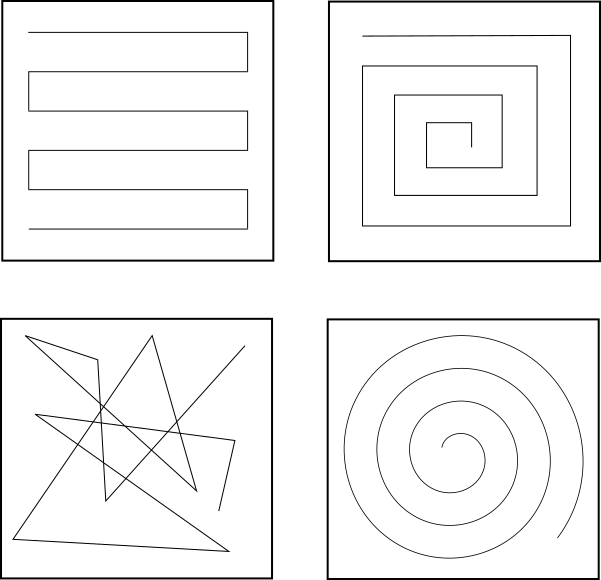
\includegraphics[width=0.7\textwidth]{various_coverages_1}
\caption{Various dynamic coverage patterns}
\label{fig:covTypes}
\end{figure}

In \cite{MannadiarR10} a new algorithm based on the Boustrophedon cell decomposition is introduced. The presented algorithm encodes the areas (cells) to be covered as edges of the Reeb graph. The primary contribution of their algorithm is using the solution to the CPP in order to find the optimal order, in terms of distance travelled, in which the cells are covered. Then, given the Reeb graph an \emph{Euler tour} is calculated, that is a circuit that covers every edge in a graph exactly once. To cover the interior of a the cell a simple back-and-forth motion is used. The experiments were carried out by simulating a Pioneer robot to perform coverage of all the available free space, in different classes of environments as test cases.

In \cite{Naftos:1992} the \emph{Watchman Route Problem} (WRP) is investigated, that is: find a shortest route such that each point in the polygon $P$ is $d$-visible (i.e., visible and at most $d$ away) from some point along the route. For simple polygons when there is a visibility range $d$ and we are interested in viewing the whole interior of $P$. Two versions of the WRP are presented: find a shortest route such that either \emph{(a)} each point in the boundary of the polygon (d-watchman problem) or \emph{(b)} each point in the polygon ($d$-sweeper problem), is $d$-visible. An approximation algorithm for the TSP in simple grids is proposed, that obtains solutions within 33\% of the optimum. This also provides approximate solutions for the $d$-sweeper problem.

For the class of online algorithms, the most common approaches will be discussed  in greater detail in the body of the thesis, but let's firstly go briefly through all of them.
The simplest online algorithm is the so called \emph{Node Counting}. Basically this algorithm counts the number of visits in the various positions of the terrain to be covered and at each step chooses to go to the location with the smaller number of visits.

In \cite{Ishida:1998:RSA:608597.608621} can be found a good review of the \emph{LRTA*}. The logic behind this algorithm is similar to the Node Counting one, but in this case the value associated to a map position is not just its visit count but a cost value that is used to guide the robots near the unvisited locations. For a comparison between Node Counting and LRTA* see \cite{koenig2001}.

In \cite{Koenig96easyand} the \emph{Edge Counting} algorithm is presented. In this case the count used for making decisions is the edge traversal count of the departing links, from the current position, to the next reachable ones. Random walks are bad search algorithms since they do not remember were they have already searched but it be can easily derived a real-time search algorithm that shares many properties with random walks, but has finite complexity - basically, by “removing the randomness” from random walks. In \cite{506507}, is proved that edge counting always reaches a goal state with a finite number of action executions, but its complexity can be exponential in the size of the state space.

In \cite{5711675} the \emph{PatrolGraph*} algorithm is introduced. It takes into account both the number of visits and as node count and the edge traversals. The algorithms has been specifically designed to solve the problem of Multi–Robot Controlled Frequency Coverage (MRCFC), in which a team of robots are requested to repeatedly visit a set of pre–defined locations of the environment according to a specified frequency distribution. It is proven to
be statistically complete as well as easily implementable on real, marketable robot swarms for real–world applications.In this thesis we will exploit the properties of this algorithm to perform a Multi–Robot Uniform Frequency Coverage (MRUFC), so that all the locations of the map will be visited uniformly.


\subsection{Space Decomposition}
\label{sec:spaceDec}

To perform a path planning and define a metric for deciding when a coverage is complete we have to sub-sample the space using a methodical approach. The most common approach is to apply a so called \emph{cellular decomposition} to the space. A mathematical definition of cellular decomposition is given in definition \ref{cellDec}.

\theoremstyle{definition}
\begin{definition}{\textbf{\textit{Cellular decomposition}}}\label{cellDec}
In geometric topology, a cellular decomposition $G$ of a manifold $M$ is a decomposition of $M$ as the disjoint union of cells (spaces homeomorphic to n-balls $B_n$).
\end{definition}

Practically a cellular decomposition is a data structure that encodes the topology of a given environment, using elementary non-overlapping regions of terrain of known geometry such that adjacent cells share a common boundary and that the union of all cells coincides with the environment. The main purpose of the decomposition is to derive an abstract description of the free space, i.e., the one in which the robot can move. Moving from cell to cell and covering the space in each cell for all of them will result in covering the entire region.
\clearpage
\noindent We can distinguish two types of cellular decomposition:
\begin{enumerate}
\item Exact cell decomposition (topology-dependent)
\item Approximate cell decomposition (topology-independent)
\end{enumerate}


In the exact cell decomposition the topology of the environment is accurately represented and to accomplish this all the cells does not have to be the same size, but they contain only free space. The method also requires a complete description of the objects and a complex cell construction.  In approximate cell decomposition, the entire region is divided into equal sized cells. Any cell with any part of an obstacle in it is marked as invalid workspace. The cells do not necessarily have to be marked as empty or full, but can be represented by a fraction of the portion occupied. The approximation can be improved by increasing the resolution but this of course will increase the memory requirements if the entire grid is stored in memory. After the cells are created an adjacency graph can be produced where each vertex represents a cell and the edges represents the adjacency relationship between the cells. Then this adjacency graph is used by the algorithms to perform the path planning in order to complete the coverage.

In \cite{846365} the authors present some new examples of exact cellular decompositions whose cells are defined by critical points of Morse functions. Cellular decompositions have been widely used for planning a path between two points in the free space, but the motivating task for the work presented in this paper is coverage. Since the Morse functions define cells with “simple” structure, a planner can then use a cellular decomposition to achieve coverage by employing simple control strategies to cover each of the individual cells in the decomposition. A simple
control strategy can be back-and-forth motions, resulting in a farming style pattern.

\input{tex/figures/cellDecomposition_types}

In \cite{choset} the Boustrophedon Cellular Decomposition is introduced (figures \ref{fig:cellDec_pic3} and \ref{fig:cellDec_pic4}). Is an exact cellular decomposition approach, for the purposes of coverage. Essentially, the boustrophedon decomposition is a generalization of the trapezoidal decomposition that could allow for non-polygonal obstacles, but also has the side effect of having more “efficient” coverage paths than the trapezoidal decomposition. Cells are formed via a sequence of open and close operations which occur when the slice encounters an event, an instance in which a slice intersects a vertex of a polygon. There are three types of events: \emph{in}, \emph{out}, and \emph{middle}. Loosely speaking, at an \emph{in} event the current cell is closed (thereby completing its construction) and two new cells are opened (thereby initiating their construction). The boustrophedon cellular decomposition is an enhancement of the trapezoidal decomposition and is designed to minimize the number of excess lengthwise motions, as described in the previous paragraph. In essence, all cells between \emph{in} and \emph{out} events are merged into one cell. The advantage of having a fewer number of cells is that to complete the coverage the number of back-and-forth boustrophedon motions can be minimized. 

\input{tex/figures/grid_types}

Regarding the approximate cell decomposition instead the logic is much simpler, since the only decision we have to make is how much we want the grid to be detailed. Then we mark as free only the cells that not contain any obstacle and all the rest as non-accessible space. In \cite{stanf:cellDec} a recursive strategy is presented where the cells are continuously subdivided until one of the following scenarios occurs: each cell lies either completely in free space or completely in the C-obstacle region, an arbitrary limit resolution is reached.
Once a cell fulfils one of these criteria, it stops decomposing. This method is also called a \emph{quadtree decomposition} because a cell is divided into four smaller cells of the same shape each time it gets decomposed.

Among the resulting grids we can distinguish between \mbox{\textit{simple grids}} (i.e., without internal holes) and \textit{non--simple grids} which do not possess \textit{local cut nodes} (i.e., nodes whose removal locally disconnects the graph induced by the grid). 


Both exact cell decomposition methods and approximate cell decomposition methods have advantages and disadvantages. The former are guaranteed to be complete, meaning that if a free path exists, exact cell decomposition will find it; however, the trade-off for this accuracy is a more difficult mathematical process. Approximate cell decomposition is less involved, but can yield similar, if not exactly the same, results as exact cell decomposition.







\section{Terminology and Notation}\label{sec:terminology}

Due to the simultaneous use of the ROS network and graph theory, I will always try to use two distinct names when referring to nodes and vertices. In particular in the ROS environment is formed of nodes and a graph has vertices.

That said, every terrain can be modelled as a undirected graph, by sampling the area using a grid.
The grid is described by a navigation graph $G_N=(V,E)$, the \emph{navigation graph}, where $V$ is a set of vertices and $E$ is a set of edges. Each edge that connects vertex $i$ to vertex $j$ is represented as $e_{ij}=e(i,j)$. Let be $N(v)$ the set of vertices adjacent (connected through an edge) to $v$. The maximum degree (number of edges incident to a vertex) of the graph $G$ will be denoted by $\Delta (G)$ and the minimum degree by $\delta (G)$.


\theoremstyle{definition}
\begin{definition}{\textbf{\textit{Eulerian State Spaces}}}\label{cellDec}
A state space is Eulerian if  there are as many actions  that leave a state as there are actions that enter the (same) state.
\end{definition}

Since an undirected edge is equivalent to one incoming and one outgoing edge, all undirected state spaces are Eulerian.

The navigation graph is better represented through a strongly connected, oriented graph $\hat{G}_N$, derived from $G_N$ by doubling all its edges and assigning them opposite directions. 
$E_i=\{e_{ij}\} \neq 0$ is the finite, nonempty set of directed edges that leave vertex $v_i \in V$.  $|E_i|$ is the dimension of the set, i.e., the number of edges departing from $v_i$.

$R=\{r_i\}$ is a set of $M$ robots. Robots are allowed to move in the workspace from $v_i$ to $v_j$ in $\hat{G}_N$ only if $e_{ij} \in E_i$, i.e., if the two vertices are adjacent. 
${\bm{\lambda}}=[\lambda_1,\cdots,\lambda_N]^T  \in \Re^N$ is a vector which describes the average visiting rate to each vertex $v_i \in S$, expressed as \textit{number of robots} per \textit{time unit}. %\Re$).
${\bm{\lambda}}^*=[\lambda_1^*,\cdots,\lambda_N^*]^T  \in \Re^N$, $0 \le \lambda_i^* \le 1$ and $\sum \nolimits_1^N \lambda_i^* =1$ is a vector which describes the prescribed frequency distribution of visits. 

Similarly to \cite{koenig2001}, the expression ``one-of $X$'' returns randomly one of the elements of $X$. The notation $succ(v,e)$ returns the vertex linked to $v$ through the edge $e$. The expression $c(v)$ represents the count value associated with to the vertex $v$, initially set to zero for all $v \in V$.

Let be $U$ a structure containing all the vertices of the graph still to be visited, i.e., the \emph{unvisited set}. At last et $\ell(\cdot)$ be the function that returns the length of a path and, in particular, let $\ell(P_i) \equiv \ell_i$ be the length of the $i-$th path.















\chapter{Work Overview}

Two main branches can be identified in the algorithms developed for the terrain coverage: online and offline search methods. This two branches can fit different needs, that are related to the type of hardware to which are applied to, i.e. micro-robots swarm or advanced-robots swarm. In particular online search is a better choice for micro-robots that have restricted computational capability since they only have to perform a search on adjacent cells and make simple comparison choices. The optimisation algorithms implemented instead require a discrete computational capability since they analyse all the graph and compute many the possible combinations before taking the choice.

\noindent In this thesis work the following methods have been investigated:

\begin{itemize}
\item Online Algorithms
	\begin{enumerate}
	\item Node Counting	
	\item Learning Real-Time A*
	\item Edge Counting
	\item PatrolGRAPH*
	\end{enumerate}

\item Offline Algorithms
	\begin{enumerate}
	\item VRP Greedy Nearest Neighbour
	\item VRP Greedy A*
	\item VRP Greedy with Floyd-Warshall
	\end{enumerate}
\end{itemize}
From now on, for convenience, we will refer to the Learning Real-Time A* as LRTA*, and in the VRP Greedy we will frequently omit the \emph{greedy} attribute.

The way the algorithms operate allow to classify them also in two other classes: \emph{distributed} and \emph{centralised} algorithms. In fact, while in the real-time algorithms the quadcopters are autonomous and compute their paths while moving, the optimised algorithm require a central brain that calculates the optimal paths and send them to the quadcopters. Nevertheless a distributed version of the optimised algorithm is possible to implement by distributing the evaluation of the algorithm among the robots.
In the next two chapters both types of algorithms will be discussed in depth, providing a detailed explanation, pseudo-code of the algorithm, images of the generated ROS graph network and sample screen-shots of the simulator at the end of the coverage (trails are left by the quadcopters while moving).

\begin{figure}[H]
\centering
\includegraphics[width=\textwidth]{simulation_environment}
\caption{The 3D simulation environment}
\label{fig:simEnv}
\end{figure}


To test the algorithms the 3D simulation environment was created from scratch using the VREP robotic simulator (Fig. \ref{fig:simEnv}). The map has been created trying to include a variety of topology characteristics, such as: dead ends, loops and open-spaces.
As stated in the first chapter the environment map is sub-sampled using a regular grid, and a binary value is assigned to every cell of the grid: \textbf{0} represent an accessible cell, while \textbf{1} represents an occupied cell, as shown in Fig. \ref{fig:mapGrid}.  There exists a vertex $v \in V$ for every cell of the grid, and every vertex $v$ is connected to its accessible adjacent $w_i$ vertices with an undirected edge $e=(v,w_i) \in E$. The result, is a strongly connected graph, where every node $v$ can be reached from every vertex $w$ directly, or by traversing a finite number of vertices. The edge cost is simply calculated using the euclidean distance. The edge connecting two neighbours has always the same cost. Nevertheless a possible extension can be applied in the search methods using the A* path finding algorithm \cite{4082128}. The matrix used by the A* in fact is not binary. To an accessible cell instead, a value from 0 to 5 can be assigned, which represents the cost of travelling across that particular cell. Zero means the least possible difficulty in travelling whilst five represents the most difficult, .


%\begin{figure}[H]
%\centering
%\includegraphics[scale=0.4]{map_grid}
%\caption{The binary access matrix built on top of the 3D environment}
%\label{fig:mapGrid}
%\end{figure}

\begin{figure}[H]
  \begin{minipage}[b]{0.45\linewidth}
    \centering
\includegraphics[scale=0.4]{map_grid}
\caption{The binary access matrix built on top of the 3D environment}
\label{fig:mapGrid}
    %\vspace{4ex}
  \end{minipage}
\quad
  \begin{minipage}[b]{0.45\linewidth}
    \centering
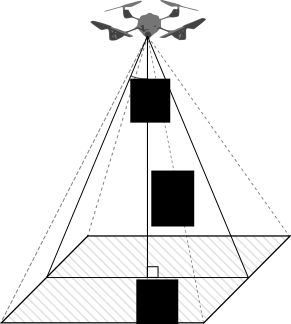
\includegraphics[scale=0.7]{quad_fov}
\caption{Scheme for the calculation of the view surface}
\label{fig:quadFov}
   % \vspace{4ex}
  \end{minipage}
\end{figure}

From Fig. \ref{fig:quadFov} we can see that, using downward facing cameras with a square vision sensor having a view angle of $2\alpha$ mounted on the hovering robot flying at height $h$, the side $b$ of the projected square that defines the view surface can be calculated as:
\begin{equation}
b = 2(h \tan(\alpha))
\label{eq:viewSide}
\end{equation}
So following formula \ref{eq:viewSide} we can set the flying height $h$ such that a cell, of side $b$, is completely covered. 
The input of the coverage solver is then a simple text file containing the occupancy grid matrix. The coverage planner will store the vertices of the graph as a vector of structs (C++ standard template library) associating the \emph{position}, \emph{occupancy} and \emph{visit count} properties as in Fig. \ref{fig:graph_struct}, and a separate adjacency graph so to apply all the discussed algorithms. In this way it's really easy to describe a terrain so that having for example just an image of a geographic area we can easily convert it to an occupancy grid using some dedicated software manually or automatically. We can observe anyway that not-accessible cells of the map will never be taken into account by the algorithm since no edge points to them, but they will still occupy memory space. That's why an alternative input method has been provided for the controllers, consisting in a map already represented as an adjacency graph but containing only the accessible vertices, with an auxiliary file specifying the position in the space for each vertex. Using this representation of course the process of converting a raw image to a consistent graph becomes a little bit more complex and for small maps the reading time and memory allocation space may not vary significantly, but with bigger and more detailed maps the advantages may become considerable. The grids in Fig. \ref{fig:grid1} and Fig. \ref{fig:grid2} for example are represented using adjacency graphs.

\begin{figure}[H]
\centering
\includegraphics[scale=0.6]{graph_structure}
\caption{Graph structure}
\label{fig:graph_struct}
\end{figure}

\section{The way-point planning algorithm}

The basic mechanism used to move the quadcopters relies on the fact that in the simulator, to each quadcopter is associated a so called manipulating sphere, shortly the MP, which the quadcopter follows whenever the sphere centre does not coincide with its centre. It comes natural then to understand that the \emph{quad} controllers move this spheres to manipulate the robots in the environment. 
While performing the coverage the quadcopters move only from one vertex to a neighbour one and, under this condition no obstacle can be found if the map is accurate enough. Anyway a short remark has to be done about this: since the control algorithm embedded in the quadcopter of the V-REP simulator is (as stated by the algorithm's author) ``quickly written and is dirty and not optimal'', an additional path planning was developed beneath the search algorithms.
In particular if the MP is placed too far away, the thrust given to the propellers of the quadcopter, being directly proportional to the distance MP$\rightarrow$quadcopter, becomes too high. This causes the quadcopter to become highly unstable and eventually lose control and crash. To overcome this problem a `critical distance' has been defined, and if the MP$\rightarrow$quadcopter distance is greater then the critical one, intermediate way-points are dynamically interpolated to safely guide the quadcopter to the target.
So combining this necessity with the one of following a given path vertex by vertex, a waypoint follower algorithm was developed with the logic shown in Fig. \ref{fig:wp_flowch}.


\begin{figure}[t]
\centering
\includegraphics[width=\textwidth]{way-point_flowch}
\caption{The flow-chart of the inter-vertex trajectory planning}
\label{fig:wp_flowch}
\end{figure}

In the flow-chart the way-points relative to a vertex are called targets, while the \mbox{way-points} between two vertices are called sub-targets. The distance between a quadcopter and the target is called \textit{dist} while the distance between a quadcopter and a sub-target is called \textit{subDist}. The critical distance mentioned above is shortened as \textit{CRIT\_DIST}.
This argumentation does not apply to the control of the real quadcopter since the platform used for the experiments on the field. an Asctec\textsuperscript{TM} Pelican has a very good PID controller (better described further on) for which the targets are just sent without sub-path-planning.

All this control logic is contained within a bigger one where we check whether we acquired the quadcopter position (needed for all the distance comparisons) and if we have completed the coverage.

\chapter{Online Algorithms}

When dealing with swarms of robots the biggest branch of studies and experiments on this topic usually refers to little robot units with limited sensing, and limited computational capabilities. In this framework simple real time search methods play a significant role since, even if the behaviour of the algorithm itself is not sophisticated, groups of robots take advantage of their collective behaviour, parallelism and fault tolerance. \\
A key concept in swarms behaviour is \emph{stigmergy}, concept at the base of the path planning used in the developed real-time search algorithms.  The stigmergy mechanism allow multiple agents to coordinate indirectly by leaving traces of their movements in the environment. This kind of mechanism is the same used by ants:~they communicate using pheromones trails that are laid and can be followed by other ants. The more ants follow a trace, the more they refresh the pheromone left, and so other ants will follow that path more likely.

We apply the same concept but somehow in a reversed fashion. The terrain is modelled as a grid divided in cells and, since our objective is to perform a complete coverage of the grid, we make our choice by looking at the less visited cells and moving onto them. Both Node Counting and the LRTA* share the same operative work-flow which is synthesised in the following pseudo-code:

\begin{algorithm}
\caption{Navigation Algorithm for the real-time search}
\label{alg:rt_gen}
\begin{algorithmic} [1]
\STATE{$v_c = v_{start}$} \label{a:init_v}
\STATE{$U \leftarrow$ \emph{``set of unvisited vertices''}} \label{a:initU_rt}
\WHILE{$U \neq \emptyset$}\label{a:bigWhile_rt}
	\STATE{$e = choose(v_c, Alg)$} %\COMMENT{$Alg$ determines how the edge is selected.}}
	\STATE{move along edge $e$} %\COMMENT{the robot moves in the Workspace.}}
	\STATE{$v_c := succ(v_c, e)$}
\ENDWHILE
\end{algorithmic}
\end{algorithm}

The three search methods differ only in the \emph{choose} rule which will be discussed in the next sections. The pheromone mechanism is implemented by embedding a count-grid in each agent which is updated by means of the ROS network: each node is at a same time publishing and subscribed to the same common topic  \textit{updateLRTACount}, and each time one of the agents publishes on it, all of them updates the counts in their grid.

Let's go through the algorithm: at the beginning a start vertex is assigned (line \ref{a:init_v}) to each quadcopter, and the set $U$ of unvisited vertices is initialised (line \ref{a:initU_rt}). In particular the unvisited set contains all the vertices in the graph with a key value of 0, representing the accessible cells. From this vertex all the neighbour vertices $w_i$ are tested looking at its $c(w_i)$ associated value. We can observe that this methods do not require any memory, since the update rule is just related to the vertex the robot is visiting at a given time and not on the history of its path.

\begin{figure}[t]
\centering
\includegraphics[scale=0.3]{swarm_LRTAstar}
\caption[ROS network for the online algorithms]{The nodes and topics ROS network of the online algorithms. The ellipses are nodes while the rectangles are topics.}
\label{fig:rt_nodes}
\end{figure}

All the control \emph{quadLRTAstar} nodes are launched together using the \texttt{roslaunch} package. Each time a robot is about to move it check whether all the nodes have been visited, and if the unvisited set is empty the robots stop searching.
As you can see in figure \ref{fig:rt_nodes} all the ROS nodes are independent, but they communicate through the common topic. This node network is relative to the LRTA* algorithm, but the same scheme holds also for all the other online algorithms.

If a robots find itself in a situation where two adjacent vertices happen to have the same value of interest, whether this is a vertex count (Node Counting), an heuristic estimate (LRTA*), and edge count (Edge Counting) or an edge transition probability (PatrolGRAPH*), the robots chooses randomly one of the equally best values. For the multi-robot coverage due to possible communication delays the random factor plays a significant role in spreading out the robots across the map, decreasing the total coverage time.




\section{Node Counting}

Following the logic described in the previous algorithm (\ref{alg:rt_gen}), the Node Counting search updates the vertex count using the following simple rule:

\begin{algorithm}
\begin{algorithmic}[1]
\STATE{$w =$ one-of $arg min_{w_i \in N(v_c)} c(w_i)$} \label{a:find_next_nc}
\STATE{$c(v_c) = 1 + c(v_c)$}\label{eq:nc_rule}
\RETURN{$e(v,w)$}
\end{algorithmic}
\caption{\emph{Choose} operator for Node Counting}\label{alg:rt_nc}
\end{algorithm}


At the beginning of time all the vertices start with a count $c(v)=0$, which means that they are all unvisited vertices. While the robots are exploring the area the Node Counting search make the robots move to the nearest neighbour vertex with the smallest count, so that the swarm agents are automatically steered to the closest unvisited zones. In this way after some time all the vertices will be visited.

\section{Learning Real-Time A*}
\label{sec:LRTAstar}

The update rule of the node Learning Real-Time A* is a little bit less trivial, since is not only based on the current vertex, but also on the successor. The LRTA* algorithm repeats the following steps until the problem solver reaches the goal state. It builds and updates a table containing heuristic estimates of the cost from each state in the problem space. Initially, the entries in the table come from a heuristic evaluation function, or are set to zero if no function is available, and are assumed to be lower bounds of actual costs. Through repeated exploration of the space, however, more accurate values are learned until they eventually converge to the actual costs to the goal \cite{Ishida:1998:RSA:608597.608621}. Its complexity is found to be a small polynomial in n (number of states) \cite{Koenig96easyand}. The vertex count is updated as follows:

\begin{algorithm}
\begin{algorithmic}[1]
\STATE{$w =$ one-of $arg min_{w_i \in N(v_c)} c(w_i)$} \label{a:find_next_lrta}
\STATE{$c_{_{LRTA}}(v) = 1 + c_{_{LRTA}}(w)$}\label{eq:lrta_rule}
\RETURN{$e(v,w)$}
\end{algorithmic}
\caption{\emph{Choose} operator for LRTA*}\label{alg:rt_lrta}
\end{algorithm}

Let's remark first of all that the $c_{_{LRTA}}$ count for this algorithm is not the actual number of visits but an heuristic estimate used for the choosing phase. At the beginning of time all the vertices start with a count $c=0$, which means that they are all unvisited vertices. To understand the mechanism of the LRTA* search, let's imagine to be able to look at a snapshot of the vertices count in the middle of a coverage execution: the $c_{_{LRTA}}(v)$ count value of a vertex $v$ represents the distance from this vertex $v$ to the closest vertex $w$ with $c_{_{LRTA}}(w)$, e.g. an unvisited vertex in a single-coverage case. Since the logic that guides the agent is always to look at the neighbouring vertices with the smallest count, the robot will not only be steered towards the nearest unvisited vertices, but in doing that they will also follow an approximately shortest path.
In \cite{koenig2001} is demonstrated how the LRTA* exhibit better performances than Node Counting for that while in the latter the cover time can be up to exponential in the number of vertices in the graph, the former guaranteed the coverage to be completed in a time polynomial to the number of vertices in the graph.

Despite this the extension of this property from the single-robot case to a multi-robot one is not straightforward and the experimental results for a single-visit coverage show how in some cases Node Counting can be more efficient. This behaviour is related to the update-count rule: while in NC a robot can communicate its vertex choice and consequently update the vertex count in the very same moment he chooses, for the LRTA* a robot has first to reach the vertex and only then it can update its count (since it's related to its next vertex choice). Due do this in LRTA* if many robots are on the same vertex nothing stops them from choosing all the same next vertex, yielding to an inefficient coverage. For single-robot coverage of course this problem does not occur. 


\section{Edge Counting}
The Edge Counting algorithm the count used for making decisions is the edge traversal count of the departing links, from the current position, to the next reachable ones. Supposing we are in vertex $v_c$ where $e_{cj} \in E_c$ form the set of its outgoing edges, the choose operator for this algorithm is:

\begin{algorithm}
\begin{algorithmic}[1]
\STATE{$l =$ one-of $arg min_{j : e_{cj} \in E_c} k_{cj}$} \label{a:find_next_ec}
\STATE{$k_{cl} =k_{cl} + 1$}\label{eq:ec_rule}
\RETURN{$e(c,l)$}
\end{algorithmic}
\caption{\emph{Choose} operator for Edge Counting}\label{alg:rt_ec}
\end{algorithm}

$k_{ij}$ is the edge count, an integer variable initialized to $0$ which counts the number of times that robots have chosen to proceed to $v_j$ after leaving $v_i$. In general, no real-time search algorithm can beat the complexity of LRTA*, which is a small polynomial in n. In contrast, the deterministic Edge Counting that we derived from random walks has a complexity that is at least exponential in n. The picture changes in Eulerian state spaces. The complexity of edge counting decreases dramatically and equals the complexity of LRTA*, which remains unchanged (it even beats LRTA* in certain specific domains) \cite{Koenig96easyand}. 


\section{PatrolGRAPH*}

The logic behind the PatrolGRAPH* follows a different approach. First of all, although it is presented as online algorithm, it also presents an offline phase which is needed in order to optimise the successive online phase. So we can classify it in the middle of the two approaches. It takes into account not only information about the vertex count, but also on the edge traversal count. In particular the decision that is made in vertex $v_i$ to choose the next vertex $v_j$ is based on the probability associated to the edge that connects them $e(i,j)$.
The algorithm is designed to solve the problem of Multi--Robot Controlled Frequency Coverage, in which a team of robots are requested to repeatedly visit a set of pre--defined locations of the environment according to a specified \emph{frequency distribution}. In particular we want the frequency distribution to be \emph{uniform} in order to visit all the vertices of the graph in the shortest time, and this kind of formulation is known as the Multi--Robot Uniform Frequency Coverage (MRUFC). In particular the MRUFC problem corresponds to the case when ${\bm{\lambda}}^*$ has a uniform distribution, i.e., for all $s_i$, $\lambda_i^* = 1/N$.  The frequency distribution of visits in particular is controlled by tuning the so called \emph{transition matrix} $P$, which contains for each edge $e_{ij}$ the probability $p_{ij}$ of being traversed. $P$ is subject to the following constraints:

\begin{equation}
\sum\limits_{j=1}^{N} {p_{ij} } = 1, \quad (i=1,\ldots,N),
\label{Pmatrix3b}
\end{equation}

\begin{equation}
0 \leq p_{ij} \leq 1,\quad (i,j=1,\ldots,N). 
\label{Pmatrix3c}
\end{equation}
 
   In its simplest form the elements of $P$ will be:

\begin{equation}
p_{ij}=\frac{1}{|E_i|},
\label{eq_adj}
\end{equation}
if $v_i$ and $v_j$ are adjacent, while if $s_i$ and $s_j$ are not adjacent,
\begin{equation}
p_{ij}=0.
\label{eq_noadj}
\end{equation}

It is easy to understand that with this kind of formulation every vertex will receive a number of visits which is proportional to its incoming edges, and we want instead all the vertices to be visited uniformly. To accomplish this the PatrolGRAPH* performs the so called \emph{offline phase} to tune the $P$ transition matrix.

\subsection{The offline phase}


Let $\bm{1}=[1 \ldots 1]^T$ be the unitary vector. The flow balance equations in matrix form, by considering the additional requirement that the sum of average visiting rates, computed over all vertices of $\hat{G}_N$, is constant, can be written as:

\begin{equation}
\left[\begin{array}{*{20}c} {P^T - I} \\ {\bm 1^T} \end{array} \right] \bm \lambda = \left[\begin{array}{*{20}c} {0} \\ \vdots \\ {0} \\ {C} \end{array}\right].
\label{theorem45}
\end{equation}

The system \eqref{theorem45} has exactly one solution whenever $P$ is stochastic and irreducible \cite{5711675}. The last equation in \eqref{theorem45} allows one to determine the unique solution whose components sum up to $C$.

The off--line phase then has the main purpose of finding a solution to the so--called \emph{inverse problem}, i.e., the problem of choosing $P$ such as to guarantee that the solution of \eqref{theorem45}, with $C=1$, corresponds to the prescribed frequency distribution. The off--line phase does not involve the individual robots.

Let ${\bf{b}} = [b_{1}\cdots b_{N^2}]^T\in \Re^{N^2}$ be defined as a vector which parametrize the elements of the transition matrix $P$, so that $P=P({\bf{b}})\in\Re^{N\times N}$. This is done by ideally subdividing $\bf{b}$ into $N$ vectors with length $N$, and by stacking them onto each other to build up the rows of $P$. More formally, 
\begin{equation}
p_{ij}=b_{N \times (i - 1) + j}, \quad (i,j=1,\ldots,N),
\label{ths0}
\end{equation}

and $\bm{\lambda^*}$ represent the ideal desired solution of the MRCFC problem. Then, ${\bm{\lambda^*} - \bm{\lambda}({\bf{b}})}$ is a representation of the mismatch between the actual frequency distribution and the desired one as a function of the structure of the navigation graph (expressed by the entries of matrix $P$). 

The off--line phase of the \textit{PatrolGRAPH*} algorithm is the search for a solution to the following minimization problem with respect to the unknown variable ${\bf{b}}$.


\begin{equation}
{\bf{b^*}} = \arg \min_{{\bf{b}}}({\bm{\lambda^*} - \bm{\lambda}({\bf{b}})})^T ({\bm{\lambda^*} - \bm{\lambda}({\bf{b}})}),
\label{ths3}
\end{equation}
\indent subject to
\begin{equation}
\sum\limits_{j=1}^{N} {b_{N\times(i-1)+j} } = 1, \quad (i=1,\ldots,N), \\
\label{con3a}
\end{equation}
\begin{equation}
b_{N\times(i-1)+j} \ge  |\epsilon |,\quad (\forall i,j\quad s.t.\quad a_{ij} \in A_i),  
\label{con3b}
\end{equation}
\begin{equation}
b_{N\times(i-1)+j} = 0,\quad (\forall i,j\quad s.t.\quad a_{ij} \notin A_i). 
\label{con3c}
\end{equation}



\subsection{The online phase}
After performing the previous steps, the online phase follows the same pattern of the previous ones as in Algorithm \ref{alg:rt_gen}, but now the choose operator is more elaborated:

\begin{algorithm}
\begin{algorithmic}[1]
\STATE{$c(v) = c(v) + 1$} \label{a:PG_upd_cv}
\FORALL{$j$ such that $e_{cj}\in E_c$} %\label{a:initU_rt}
	\STATE{$\Delta p_{cj} = (k_{cj}- \eta_{j})/v_c - p_{cj}$}\label{a:PG_deltaP}
\ENDFOR
\STATE{$l = arg min_{j}( \Delta p_{cj})$}\label{a:PG_find_min}
\STATE{$k_{cl} = k_{cl} + 1$}\label{a:PG_upd_k}
\RETURN{$e_{cl}$}
\end{algorithmic}
\caption{Choose operator for PatrolGRAPH*}\label{alg:rt_pg}
\end{algorithm}

Where: $c(v)$ same as before is the vertex count. $k_{ij}$ is the edge count. $\eta_j$ is a zero mean random variable with standard deviation $\sigma$, that is, $\eta_j=N(0,\sigma)$. In particular $\eta$ is used to purposely introduce a factor of unpredictability but since we don't need this feature we will simply set it to zero. Line \ref{a:PG_upd_cv} updates the number of visits $c(v)$ received by $v_c$; Line \ref{a:PG_deltaP} computes, for every adjacent vertex, the error $\Delta p_{cj}$ between the ratio $k_{cj}/v_c$ and the desired relative frequency $p_{cj}$; Line \ref{a:PG_find_min} picks the edge $a_{cl}$ for which $\Delta p_{cj}$ is minimum; Line \ref{a:PG_upd_k} updates $k_{cl}$. 
In \cite{5711675} is demonstrated that the routing policy adopted by \textit{PatrolGRAPH*} in Algorithm \ref{alg:rt_pg} to distribute robots along edges $a_{ij}$ departing from $s_i$ converges to the desired relative frequencies $p_{ij}$.

To demonstrate the effectiveness of the offline phase of the PatrolGRAPH* I've tested the algorithm on a 5x5 grid obstacle-free map using 3 quadcopters, running 4 simulations with the following parameters: 
\begin{itemize}
\item No offline phase, 10 minutes patrolling (Fig. \ref{fig:PG_pic1})
\item With offline phase, 10 minutes patrolling (Fig. \ref{fig:PG_pic2})
\item No offline phase, 20 minutes patrolling (Fig. \ref{fig:PG_pic3})
\item With offline phase, 20 minutes patrolling (Fig. \ref{fig:PG_pic4})
\end{itemize}

The figures mentioned in the list are a graphical representation of the visit count for the cells in the map. In particular the visit count is encoded as a colour and the colour-bar is the reference. First of all it is important to know that the starting point for all the quadcopters is the cell in position (2,0), and this of course affects the propagation of visit in the neighbouring cells. In Figure \ref{fig:PG_pic1} and \ref{fig:PG_pic3} we can observe how without running the offline phase the corner vertices, which have the lowest number of in-going edges, receive a significantly smaller amount of visits (colour near blue).  In Figure \ref{fig:PG_pic2} and \ref{fig:PG_pic4}, instead, we notice how the visit distribution is much more uniform, and as the simulation time increases the coverage becomes more uniform.
~\\
\begin{figure}[h] 
  \label{fig:PG_countMaps}
  \centering
  \begin{minipage}[b]{0.45\linewidth}
    \centering
    \input{img/tikzPlots/5x5_unoptim_10min.tikz}
    \caption{Unoptimised PG* 10 min}
    \label{fig:PG_pic1}
    \vspace{4ex}
  \end{minipage}
  \quad
  \begin{minipage}[b]{0.45\linewidth}
    \centering
    % This file was created by matlab2tikz v0.4.7 running on MATLAB 8.0.
% Copyright (c) 2008--2014, Nico Schlömer <nico.schloemer@gmail.com>
% All rights reserved.
% Minimal pgfplots version: 1.3
% 
% The latest updates can be retrieved from
%   http://www.mathworks.com/matlabcentral/fileexchange/22022-matlab2tikz
% where you can also make suggestions and rate matlab2tikz.
% 
\begin{tikzpicture}

\begin{axis}[%
width=.75\linewidth,
%height=3.565625in,
axis on top,
%scale only axis,
xtick={0,1,...,4},
ytick={0,1,...,4},
xmin=-0.5,
xmax=4.5,
y dir=reverse,
ymin=-0.5,
ymax=4.5,
colormap/jet,
colorbar,
point meta min=0,
point meta max=18
]
\addplot [forget plot] graphics [xmin=-0.5,xmax=4.5,ymin=-0.5,ymax=4.5] {img/tikzPlots/5x5_optim_10min.png};
\end{axis}
\end{tikzpicture}%
    \caption{Optimised  PG* 10 min}
    \label{fig:PG_pic2}
    \vspace{4ex}%%
  \end{minipage}
  \begin{minipage}[b]{0.45\linewidth}
    \centering
    \input{img/tikzPlots/5x5_unoptim_20min.tikz}
    \caption{Unoptimised  PG* 20 min} 
    \label{fig:PG_pic3}
    \vspace{4ex}
  \end{minipage}
  \quad
  \begin{minipage}[b]{0.45\linewidth}
    \centering
    \input{img/tikzPlots/5x5_optim_20min.tikz}
    \caption{Optimised  PG* 20 min}
    \label{fig:PG_pic4}
    \vspace{4ex}%% 
  \end{minipage} 
\end{figure}








\chapter{Offline Algorithms}

To solve the coverage problem in an optimised fashion the problem was approached as Vehicle Routing Problem, shortly VRP, using a greedy strategy which will be discussed in depth in the next paragraphs. In this case the paths are preprocessed and the robots are guided by a central ROS node which compute the optimal path. The central node is called \emph{kernelNode} and as you can see in figure \ref{fig:nonrt_nodes} it communicates with all the quadcopter controllers through two topics: \emph{quadCtrlSignal} and \emph{pathCompleted}. Same as the before all the nodes are launched together using the \texttt{roslaunch} package, but the \emph{quadcopterRosCtrl} nodes are not able to publish their position commands until the \emph{kernelNode} is done computing the paths. Only then the central node triggers the ``start'' command, and the control nodes start moving the quadcopters. When a quadcopter finishes to follow its path, it publish a message over the \emph{pathCompleted} topic. When all the quadcopters are done, the central node stops triggering the control signal and the ROS network is shut down.


\begin{figure}[h]
\centering
\includegraphics[scale=0.3]{swarm_Greedy}
\caption[ROS network for the offline algorithms]{The nodes and topics ROS network of the offline algorithms. The ellipses are nodes while the rectangles are topics.}
\label{fig:nonrt_nodes}
\end{figure}

The power of this algorithm is that the paths created are cycles so that at the end of the execution all the robots are back in the beginning position, which can be useful from a logistic point of view in a urban search and rescue application, and it's convenient from an energetic point of view. For a survey on \textit{green} VRP see \cite{greenVRP}. To get to the final version of the VRP Greedy I went through some intermediate solutions that I will describe in the following section to show the evolution of algorithm. The first version was just using nearest neighbour nodes when constructing the path, but in a multi-robot approach this turned out to be highly inefficient. So the A* algorithm came in to take into account all the vertices still to be inserted and using the shortest path algorithm to find a way to non-neighbouring vertices. But when increasing the size of the maps computing the A* algorithm each step of the Greedy alg. became time consuming. So finally, since the map is known a priori the Floyd-Warsall algorithm became the most natural solution to find the shortest paths between all pair of vertices at once and this drastically increased the execution time.


%\setcounter{section}{1}
\section{$\min \max$ Vehicle Routing Problem}
\label{s:vrp}

Let's consider the problem of exploring an area with a swarm of quadcopters.


Let $d_{vw}$ be the distance between the vertex $v$ and the vertex $w$.
We can assume that $d_{vw}$ is the euclidean distance between the centre of the cell corresponding to the vertices  $v$ and $w$.
Let $F = \{ 1, \ldots, i, \ldots, N\}$ be the set of quadcopter and let $s_i$ be the starting vertex  of the quadcopter $i$.
A path $P_i$ is assigned to each quadcopter, consisting in an ordered sequence of vertices of $V$ to be visited.
In particular the path of each quadcopter $i$ starts in $s_i$ and ends in $e_i$.
Let $\ell(\cdot)$ be the function that returns the length of a path and, in particular, let $\ell(P_i) \equiv \ell_i$ be the length of the $i-$th path.

The problem consist in planning the trajectories such that:

\begin{enumerate}[label=\textbf{\arabic*.}]
\item the distance travelled by  the quadcopter with the longest path is minimized

\item every vertex is visited at least once
\end{enumerate}

In symbols:
\begin{equation}
\min \quad \mathcal{L} \label{e:obj}
\end{equation}
subject to:
\begin{equation}
\mathcal{L} \geq \ell(P_i) \quad \forall i \in F \label{e:max}
\end{equation}
\begin{equation}
v \in \cup_{i \in F} P_i \quad \forall v \in V \label{e:allIncluded}
\end{equation}


Where \eqref{e:obj} is the \textit{objective function},
the constraints \eqref{e:max} impose $\mathcal{L}$ as maximum length and
the constraints \eqref{e:allIncluded} impose that every node is visited.

\section{The Greedy Algorithm}
\label{s:greedy}
The greedy algorithm is a constructive procedure that iteratively produces a solution.
At each iteration the algorithm takes an incomplete solution (potentially empty) and adds a vertex to produce a new solution.
At every step the algorithm finds the vertex $v$ to be inserted, together with the path $i$ and the position $p$ in which the vertex has to be inserted.

In particular there are two nested levels of optimisation.
The first one is path-local and, for a given robot $i$, checks among the different insertion positions $p$ of a same vertex $v$ which one generates the shortest tentative path length.
The second level of optimisation instead is global and checks among all the shortest $P_i$ paths which one generates the smallest increment with respect to the current longest path. The current length of the longest path will be identified with the letter $\mathcal{L}$.
The choice is made by testing the $\delta_{vip}$ increment in the objective function and then choosing the configuration $<v,i,p>$ that produces the smallest increment.
The complexity of the algorithm is then polynomial $O(\vert V \vert^2 N)$.

In the basic version is convenient to use a single variable $\delta$ and a single triplet \mbox{$<v,i,p>$} to be updated at every iteration. We will call $P_i^{<v,i,p>}$ the path $P_i$ modified inserting the vertex $v$ in the position $p$.
It is convenient, for an implementation point of view, to save the tentative path $P_i^{<v,i,p>}$ in a variable different from $P_i$ (it is enough just a single temporary path instead of one for each vehicle).

\begin{algorithm}[ht]
\begin{algorithmic}[1]
\STATE{$U \leftarrow V$} \label{a:initU}
\FORALL{$i \in F$} \label{a:initFor_i}
\STATE{$P_i \leftarrow \left( s_i, e_i \right) $}\label{a:initP_i}
\ENDFOR \label{a:endForiniti}
\WHILE{$U \neq \emptyset$}\label{a:bigWhile}
\STATE{$(\delta_{vip},\delta^{\text{best}}) \leftarrow + \infty$}\label{a:initDelta}
\STATE{$\mathcal{L} = \max_{\forall i \in F} \ell(P_i)$}\label{a:initBigL}
\STATE{choice $\leftarrow \emptyset$}\label{a:initChoice}
 \FORALL{$v \in U$}\label{a:forV}
  \FORALL{$i \in F$}\label{a:forI}
  \STATE{$(\ell_{i}^{\text{ min}}, \ell_{i}^{\text{ tent}}) \leftarrow + \infty$}\label{a:initLength}
   \FORALL{position $p \in P_i$}\label{a:forPos}
   \STATE{$\ell_{i}^{\text{ tent}} = \ell(P_i^{<v,i,p>})$}\label{a:updateLtent}
    \IF{$\ell_{i}^{\text{ tent}} < \ell_{i}^{\text{ min}}$}\label{a:checkLtent}
    \STATE{$\ell_{i}^{\text{ min}} = \ell_{i}^{\text{ tent}}$}\label{a:updateLmin}
    \STATE{$\delta_{vip} = \ell_{i}^{\text{ min}} - \mathcal{L}$}\label{a:calcDelta}
    \IF{$\delta_{vip} < \delta^{\text{best}}$}\label{a:testDelta}
     \STATE{$\delta^{\text{best}} \leftarrow \delta_{vip}$}\label{a:saveDelta}
     \STATE{choice $\leftarrow <v,i,p>$}\label{a:saveChoice}
    \ENDIF \label{a:endIfTestDelta}
    \ENDIF
   \ENDFOR \label{a:endForPos}
  \ENDFOR \label{a:endForI}
 \ENDFOR \label{a:endForV}
 \STATE{add $v$ to $P_i$ in position $p$} \label{a:doIt}
 \STATE{$U \leftarrow U \setminus choice.v$}  \label{a:removeV}
\ENDWHILE \label{a:endBigWhile} 
\RETURN{$P = \cup_{i \in F}P_i$} \label{a:return}
\end{algorithmic}
\caption{Greedy algorithm for the $\min \max$ VRP}\label{alg:greedy}
\end{algorithm}

Here is the algorithm in detail:
the rows \ref{a:initU}--\ref{a:initChoice} are used to initialise all the variables.
In particular the structure of $U$ is initialised (line \ref{a:initU}) with the set of all  the accessible nodes (not shown in the code: the start nodes $s_i$ are excluded).
The paths are initialised with a sequence that begins and ends with the starting nodes  (\ref{a:initFor_i}--\ref{a:endForiniti}). 
At the beginning of the main loop (line \ref{a:bigWhile}),
the variable $\delta_{vip}$, containing the increments of the objective function is initialised at plus infinite, and the same thing goes for the best increment $\delta^{\text{best}}$ (line \ref{a:initDelta}).
We then initialise $\mathcal{L}$, with the length of the longest path and reset the best choice (lines \ref{a:initBigL}--\ref{a:initChoice}).
In the next three nested loops (lines \ref{a:forV}--\ref{a:endForV}) is tested the insertion of every vertex $v \in U$ in every possible position $p$ of every possible path $i$. For a given robot $i$, the length after the insertion, called $\ell_{i}^{\text{ tent}}$, is then compared to the smallest current length among all the insertions,  $\ell_{i}^{\text{ min}}$ (line \ref{a:checkLtent}).
Note: the position to consider are the ones included between the position after the start and before the end. If the tentative length is smaller than the current best one it becomes the new best (line \ref{a:updateLmin}) and the increment is calculated with respect to the objective function previously evaluated, using the following formula:
\begin{equation}\label{e:delta}
\delta_{vip} = l_{i}^{\text{ min}} - \mathcal{L}
\end{equation}
The best $<v,i,p>$ triplet (line \ref{a:testDelta}) is saved (line \ref{a:saveChoice}) together with the corresponding increment (line \ref{a:saveDelta}).
After all the for loops are executed the best insertion is applied (line \ref{a:doIt}) and the chosen vertex is removed from the list of unvisited vertices (line \ref{a:removeV}).
When the unvisited set $U$ is empty (line \ref{a:endBigWhile}), the solution is returned (line \ref{a:return}).





\section{VRP Greedy Nearest Neighbour}

This version of the VRP Greedy follows basically the exact same scheme explained in the previous paragraph. The reason why it was called the ``Nearest Neighbour'' comes from the way it looks for the vertices. The candidates vertices to be inserted in a the path of a robot $i$ are chosen among all the vertices in the neighbouring of that robot's path $P_i$. Remember that by how we defined our graph in the first chapter (\ref{sec:terminology}), a vertex $v$ has edges that point only to its neighbours $w_i$, so any other vertex insertion would have been inconsistent. So if we are to test vertex $v_t$ in positon $p$ of path $P$ we only insert it if $e(P(p-1),v_t)=1$ and $e(P(p-1),v_t)=1$.
If we were to operate with a single robot, it always true that there exist a neighbour unvisited vertex, but this is no more valid when we deal with a swarm of robots. To solve this problem the VRP Greedy A* was developed.

\section{VRP Greedy A*}

This extension of the previous VRP make possible for the algorithm to check vertices which are not in the neighbouring of a certain $P_i$ path. When all the neighbour vertices of a certain path have been already visited, the greedy search starts looking for all the remaining vertices, and it finds a way through the graph using the A* path-finding algorithm. In particular if we consider the insertion of a vertex $v$ in a position $p$, the destination position will be between the vertex $P(p)$ and $P(p-1)$. The algorithm checks firstly whether the vertex $v$ is a neighbour of $P(p-1)$ and, if not, it calculates the so called ``\emph{way there}''. Then it checks whether the vertex $v$ is a neighbour of $P(p)$ and, if not, it calculates the so called ``\emph{way back}''. The final A* path will be then:

\begin{equation}
way there + v + way back \label{e:astarpath}
\end{equation}

To fit the behaviour of this algorithm the \mbox{$<v,i,p>$} variable was modified by introducing a fourth parameter $n$, a boolean variable which tells if the current best choice is a vertex adjacent to the corresponding $P_i$ path or not. The resulting new choice was simply called \mbox{$<v,i,p,n>$}, and a the moment of the insertion (line \ref{a:doIt} of algorithm \ref{alg:greedy}), if $n=\texttt{false}$ the A* path of will be inserted in position $i$.

The problem found with this approach was that the A* algorithm is performed every time a vertex $v$ is tested on a position $p$ and since the greedy algorithm tests all the possible configuration, on maps with more than 100 nodes the computational time started to be too big. Moreover if assume the map is not changing, which we are, there is no need of computing the shortest path every time, and that's why the next algorithm was developed.


\section{VRP Greedy with Floyd-Warshall}

The Floyd-Warshall algorithm is a method to find the lengths of the paths between all pairs of vertices. Using an auxiliary \textit{parent} structure it also possible to to get the actual path, needed for the final evaluation of the optimal coverage path. The Floyd-Warshall algorithm falls in the category of \textit{dynamic programming} since it breaks down the problem of finding a path between two arbitrarily distant vertices into simpler sub-problems.

The algorithm maintains a distance matrix ($D$) such that at iteration $k$, $d_{ij}$ is the shortest path from $i$ to $j$ using nodes 1, 2, ...$k$ as intermediate nodes. After the algorithm terminates, assuming that no negative cost cycle is present, the shortest path from nodes $i$ to $j$ is $d_{ij}$. $P$ is the parent matrix, and the meaning of its entries $p_{ij}$ is: ``for some shortest path from $i$to $j$, the vertex right before $j$ is $p_{ij}$". So given a graph $G(E,V)$, the algorithm proceeds as follows:

\begin{algorithm}[ht]
\begin{algorithmic}[1]

\STATE{$D \leftarrow G$} \label{fw_initD}
\STATE{$P \leftarrow G$} \label{fw_initP}
\FORALL{$i \in G$} \label{fw_initFor_i1}
  \FORALL{$j \in G$} \label{fw_initFor_j1}
    \relax
    \IF {$i == j \lor d_{ij} == \infty$}
    \STATE {$p_{ij} = -1$}
    \ELSE
    \STATE {$p_{ij} = i$}
    \ENDIF
  \ENDFOR
\ENDFOR
\FORALL{$i \in G$} \label{fw_initFor_i2}
      \FORALL{$j \in G$} \label{fw_initFor_j2}
	  \FORALL{$k \in G$} \label{fw_initFor_k2}
	   \STATE {$dist_{ikj} = d_{ik} +d_{kj}$}
	    \IF {$dist_{ikj} < d_{ij}$}
	    \STATE {$d_{ij} =dist_{ikj} $}
              \STATE {$p_{ij} = p_{kj}$}
	    \ENDIF
	  \ENDFOR
      \ENDFOR
\ENDFOR
\RETURN{$D$} \label{a:return_D}
\end{algorithmic}
\caption{Floyd-Warshall Algorithm}\label{alg:floydWarsh}
\end{algorithm}

We initialize all entries $p_{ij}$  to $i$ when we have an edge, and if not we set it to $-1$. The update process of the parent array basically mean the following: ``if going from $i$ to $j$ through $k$ ($i \rightarrow k \rightarrow j$) is an improvement, then we set the parent of $j$ in the new shortest path to the parent of the path $k  \rightarrow j$". To recover the path from $i$ to $j$ simply recurse on $p_{ij}$'s entries.
In this formulation inside the triple loop of the greedy solver the vertices inserted in the path are just the one in the unvisited set $U$, without all the shortest paths between not adjacent nodes. The shortest paths all inserted all at once at the end of the execution (post-insertion), and not while executing the solver (contextual-insertion). This reduces a lot the number of possible insertion positions $p \in P_i$ increasing the algorithm execution speed, but also meaning that we reduce the amount of solution space we explore. Some comparisons between result with the shortest path contextual-insertion and the post-insertion showed that there was so significant improvement to justify the former approach in favour of the latter.

In the next chapter will be presented the results obtained for the different algorithms and due to the motivation explained in this chapter the only algorithm used for the offline class will be the VRP Greedy using Floyd-Warshall.
\pagebreak






\chapter{Simulations and Results}

The five algorithms where tested on different kind of maps and compared on three major performance indexes. Since our goal is to perform the coverage in the shortest time possible, minimize the total energy spent and also don't have redundant robots that do not produce a significant contribution to the coverage, the comparison criteria are based on:
\begin{itemize}
\item  Longest path (among all the robots) - $\max(\ell_i)$
\item  Total length of paths (sum over all the robots) -  $\sum(\ell_i)$
\item  Standard deviation of the paths lengths - $\sigma(\ell_i)$
\end{itemize}

The experimental phase is divided in two sections. In the first phase we analyse the algorithms behaviour in maps with random obstacles and compare the performances. The aim is to check among the different algorithms which one performs better in each situation. In the second phase instead the aim is to identify the optimal number of robots for a given map size so all the algorithm are tested varying the number of robots. The maps considered in this second phase are obstacle-free.
For a navigation graph $G_N(E,V)$ the standard coverage is said to be completed when all the vertices have been visited at least once, in formulas:

\begin{equation}
\min_i c(v_i) \geqslant 1 \qquad \forall v_i \in V
\end{equation}

Since some online algorithms due to their nature exhibit a more efficient behaviour on multiple coverages, i.e. patrolling, these algorithms have been tested also for $\min c \geqslant C$ where $C$ is greater than one.

For the first phase on grid maps with random obstacles, let's differentiate the three types of maps used in the algorithm by defining an obstacle index $\upomega$. The reference figures are Fig. \ref{fig:obstGrid1}, Fig. \ref{fig:obstGrid2} and Fig.\ref{fig:obstGrid3}.

\begin{figure}[H] 
  \label{fig:grid_types2} 
  \begin{minipage}[b]{0.32\linewidth}
    \centering
    \includegraphics[width=0.8\textwidth]{6x6_Sparse1_1}
    \caption{$\upomega$=1}
    \label{fig:obstGrid1}
    \vspace{1ex}
  \end{minipage}
  \begin{minipage}[b]{0.32\linewidth}
    \centering
    \includegraphics[width=0.8\textwidth]{6x6_Sparse2_1}
    \caption{$\upomega$=2}
    \label{fig:obstGrid2}
    \vspace{1ex}%%
  \end{minipage}
    \begin{minipage}[b]{0.32\linewidth}
    \centering
    \includegraphics[width=0.8\textwidth]{6x6_Sparse3_2}
    \caption{$\upomega$=3}
    \label{fig:obstGrid3}
    \vspace{1ex}%%
  \end{minipage}
\end{figure}

Basically for $\upomega=0$ we have an obstacle-free map. For  $\upomega=1$ we have a map without internal holes and $\delta (G)=2$. For $\upomega=2$ we have a map with internal holes and still $\delta (G)=2$. For  $\upomega=3$ we have a map with internal holes and $\delta (G)=1$.
Tp test the algorithms the following simulation were performed:
\begin{description}
\item[\textbf{Set 1.}] Increasing map size: 4x4 Map, 6x6 Map, 8x8 Map
\item[\textbf{Set 2.}] Increasing $\upomega$:  $\upomega=1$, $\upomega=2$,  $\upomega=3$
\item[\textbf{Set 3.}] Increasing number of robots: 2 robots, 4 robots, 6 robots
\item[\textbf{Set 4.}] Increasing number of min-count per vertex: \mbox{$\min c=1$}, \mbox{$\min c =2$}, \mbox{$\min c =5$}, \mbox{$\min c =10$}
\end{description}

For each grid five different samples where tested and the result reported in the tables is the mean of the five simulations.

In the second phase to identify the best number of robots, three grid-maps of increasing size were tested, in particular the grids are: 5x5, 10x10, 15x15. For all the grids ten different simulations were performed increasing the number of quadcopters used, from a single robot coverage to a multi-robot coverage with 10 agents. In the following figures are presented 2 examples of coverage.

\begin{figure}[h] 
  \label{fig:finalPaths} 
  \begin{minipage}[b]{0.55\linewidth}
    \centering
    \includegraphics[width=\textwidth]{greedy_FW_newPlanningAlg_2}
    \caption{City map using VRP w/ F.W.}
    \label{fig:cityMap_VRP_sim}
    \vspace{1ex}
  \end{minipage}
  \begin{minipage}[b]{0.5\linewidth}
    \centering
    \includegraphics[width=0.65\textwidth]{NodeCount_10x10_10_2}
    \caption{Map 10x10 using N.C.}
    \label{fig:10x10_NC_sim}
    \vspace{1ex}%%
  \end{minipage}
%  \begin{minipage}[b]{0.5\linewidth}
%    \centering
%    \includegraphics[width=\textwidth]{LRTAStar_new_planningAlg}
%    \caption{City map using LRTA*} 
%    %\label{fig:cellDec_pic3}
%    \vspace{4ex}
%  \end{minipage}
%  \begin{minipage}[b]{0.5\linewidth}
%    \centering
%    %\includegraphics[width=0.7\textwidth]{boustrophedon_1}
%    \caption{4th path image}
%    %\label{fig:cellDec_pic4}
%    \vspace{4ex}%% 
%  \end{minipage} 
\end{figure}

\section{Algorithms Comparison}

\subsection{Single robot behaviour}
\label{sec:singleRob}
Before jumping to the multi-robot case let's make some considerations on the single-robot coverage. The extension of a single-robot coverage algorithm to the multi-robot case is not straightforward and at a first glance some of the results in the next sections may appear counterintuitive. For example as stated before LRTA* suffers a performance degradation in the multi-robot case. So, even if the scope of this thesis is focused on multi-robot coverage, to prove that the algorithms developed are fully functional and have a behaviour congruent with the result found in literature, simulations were performed also for a single-robot configuration using a 4x4 grid map. 


Since an interesting trend can be observed when changing the number of minimum visits per vertex we tested the algorithms for 4 different values of $\min c$.  The results are presented in table \ref{tab:singleRobResults}.

% Please add the following required packages to your document preamble:
% \usepackage{booktabs}
% \usepackage{multirow}
\begin{table}[H]
\centering
\begin{tabular}{@{}ccc@{}}
\toprule
Algorithm                                    & $\min c$  & $\ell(P)$           \\ \midrule
\multirow{4}{*}{Node Count} &   10        &   178             \\
                                         &   5          &     98             \\
                                         &  2           &    51              \\
                                         &  1           &    17              \\ \midrule
\multirow{4}{*}{LRTA*}     &  10          &   160             \\
                                        &   5           &   79                \\
                                        &   2           &   35                \\
                                        &   1           &   17                 \\ \bottomrule
\end{tabular}
\qquad \qquad%adds some space between tables
\begin{tabular}{@{}ccc@{}}
\toprule
Algorithm                               & $\min c$  & $\ell(P)$           \\ \midrule
\multirow{4}{*}{Edge Count} &   10      &   250              \\
                                         &   5          &     134            \\
                                         &   2          &    75               \\
                                         &   1          &   34                \\ \midrule
\multirow{4}{*}{PatrolGRAPH*}&   10   &    178            \\
                                        &   5          &   108               \\
                                        &   2          &   57                 \\
                                        &   1          &   47                 \\ \bottomrule
\end{tabular}
\caption{Single-robot comparison for a 4x4 map and $\upomega=0$}
\label{tab:singleRobResults}
\end{table}



As we can see the LRTA* always perform equal or better than Node Counting. It is interesting to notice how approaching the single coverage, the difference between NC and LRTA* becomes less considerable, becoming eventually equally for \mbox{$\min c=1$}.
Comparing Edge Count and PatrolGRAPH* we can see how for \mbox{$\min c>1$} the latter always completes the patrolling in fewer steps, while for the single coverage instead Edge Counting turns out to be more efficient. This happens since, as can be observed in appendix \ref{app:firstSteps}, in the first steps of the algorithm PG* tends to make the robot go back to already visited vertices. The reason behind this behaviour relies in the fact that having computed a Probability Transition Matrix that ensures every vertex to be visited with a probability $p=\sfrac{1}{N}$, PG* in the initial transient phase spends more time visiting vertices with a low number of edges to make coincide the desired visit frequency with the actual one.
Apart from this we can notice how the paths length for NC and LRTA* are always smaller than the ones resulting from EC and PG*, and this is also true for the multi-robot case as we will see in the next sections, making clear that vertex-count oriented algorithms are more suitable for coverage purposes.

%%%%%%%%%%%%%%%%%%

\subsection{Node Counting}

In table \ref{tab:NC_results} are presented the results for the Node Counting algorithm.

% Please add the following required packages to your document preamble:
% \usepackage{booktabs}
% \usepackage{multirow}

\begin{table}[H]
%\setlength{\tabcolsep}{1.5em}
\centering
\begin{tabular}{@{}cccccccc@{}}
\toprule
Set                & \multicolumn{4}{c}{Parameters}  & \multicolumn{3}{c}{Results}              \\ \cmidrule(lr){2-5} \cmidrule(lr){6-8}
                   & $\upomega$ & \#Rob & Grid Size & $\min c$ & $\max(\ell_i)$ & $\sum(\ell_i)$ & $\sigma(\ell_i)$ \\ \midrule
\multirow{3}{*}{1} & 1           & 3     & 4x4       &   1     &   7        &  19       &   0.394   \\
                             & 1           & 3     & 6x6       &   1     &   20      &  60       &   0.673    \\
                             & 1           & 3     & 8x8       &   1     &   37      &  109     &   0.785    \\ \midrule
\multirow{3}{*}{2} & 1           & 3     & 6x6       &   1     &   20      &  58       &  0.605     \\
                             & 2           & 3     & 6x6       &   1     &   16      &  45       &  0.625     \\
                             & 3           & 3     & 6x6       &   1     &   19      &  55       &  0.394     \\ \midrule
\multirow{3}{*}{3} & 1           & 2     & 6x6       &   1     &   27      &  54       & 0.341       \\
                             & 1           & 4     & 6x6       &   1     &   14      &  54       & 0.615       \\
                             & 1           & 6     & 6x6       &   1     &   11      &  60       & 0.770       \\ \midrule
\multirow{4}{*}{4} & 1           & 3     & 6x6       &   10     &  114	&  338       & 1.414           \\
                             & 1           & 3     & 6x6       &   5     &  68      &   202   &   0.577        \\
                             & 1           & 3     & 6x6       &   2     &  30      &  89      &   0.816       \\
                             & 1           & 3     & 6x6       &   1    &  15     &   44     &   0.816       \\ \bottomrule
\end{tabular}
\caption{Results of the simulation for the Node Counting Alg.}
\label{tab:NC_results}
\end{table}



Despite it is the simplest of the algorithms considered it is surprisingly good for multi-robot coverage. For the simulation in Set 1 of increasing map size with $\upomega=1$ the LRTA* is the only other algorithm with similar performances, although in the 8x8 grid NC still performs better. Also for Sets 2 and 3 the two algorithms get similar results, but for the 6 robots case (Set 3), the Node Counting completes the coverage in fewer steps. 

%%%%%%%%%%%%%%%%%%

\subsection{Learning Real-Time A*}

In table \ref{tab:LRTA_results} are presented the results for the Learning Real-Time A* algorithm. As stated in section \ref{sec:LRTAstar} the update-rule of LRTA* is not triggered till the robot reaches the target vertex and this entails that multiple robots can make the same choice consequently not contributing in spreading the robots across the map. This disadvantage clearly emerges from the simulations where in almost all the cases the Node Counting achieves better results. This becomes even more noticeable in Set 4 for big values of $\min c$ where even if the difference between $\max (\ell_i)$ is not that big, thinking in terms of total energy spent by the swarm, $\sum(\ell_i)$, in LRTA* is significantly bigger (NC 338 vs. LRTA* 456).

% Please add the following required packages to your document preamble:
% \usepackage{booktabs}
% \usepackage{multirow}
\begin{table}[H]
\centering
\begin{tabular}{@{}cccccccc@{}}
\toprule
Set                & \multicolumn{4}{c}{Parameters}  & \multicolumn{3}{c}{Results}              \\ \cmidrule(lr){2-5} \cmidrule(lr){6-8}
                   & $\upomega$ & \#Rob & Grid Size & $\min c$ & $\max(\ell_i)$ & $\sum(\ell_i)$ & $\sigma(\ell_i)$ \\ \midrule
\multirow{3}{*}{1} & 1           & 3     & 4x4       &   1     &  7        &  24        &   0.558   \\
                             & 1           & 3     & 6x6       &   1     &   19      &  56       &   0.773    \\
                             & 1           & 3     & 8x8       &   1     &   43      &  125     &   0.558    \\ \midrule
\multirow{3}{*}{2} & 1           & 3     & 6x6       &   1     &   23      &  68       &  0.762     \\
                             & 2           & 3     & 6x6       &   1     &   20      &  60       &  0.490     \\
                             & 3           & 3     & 6x6       &   1     &   16      &  46       &  0.840     \\ \midrule
\multirow{3}{*}{3} & 1           & 2     & 6x6       &   1     &   26      &  50        & 0.624       \\
                             & 1           & 4     & 6x6       &   1     &   19      &  72       &  0.387      \\
                             & 1           & 6     & 6x6       &   1     &   15     &   85      &   0.725     \\ \midrule
\multirow{4}{*}{4} & 1           & 3     & 6x6       &   10   &  154    &  456      &   1.633         \\
                             & 1           & 3     & 6x6       &   5     &   96     &  286      &   1.00       \\
                             & 1           & 3     & 6x6       &   2     &   31     &   91      &  0.577        \\
                             & 1           & 3     & 6x6       &   1    &    18      &  53      &  0.816  \\ \bottomrule
\end{tabular}
\caption{Results of the simulation for the LRTA* Alg.}
\label{tab:LRTA_results}
\end{table}




%%%%%%%%%%%%%%%%%%

\subsection{Edge Counting}

The first thing we notice from the results in table \ref{tab:EC_results} is that average number of visits, and consequently also total length, of the Edge Counting algorithm is generally higher for any of the 4 test cases with respect to the previous to algorithms. The results are more in line with PatrolGRAPH* algorithms ones, also for what regards the $\sigma(\ell_i)$ that in Set 4 reaches values up to $\sigma=4.08$, while for the same set the maximum for LRTA* is $\sigma=1.6$. In general it comes out that for a single-coverage task (Sets 1-2-3) on average the Edge Counting is faster than PG*.  It is worth reminding anyway that in none of the previous coverage algorithm we have control over the frequency distribution of visits, so it is not possible for example to define an ``region priority'', which can instead be achieved using the PatrolGRAPH*.

% Please add the following required packages to your document preamble:
% \usepackage{booktabs}
% \usepackage{multirow}
\begin{table}[H]
\centering
\begin{tabular}{@{}cccccccc@{}}
\toprule
Set                & \multicolumn{4}{c}{Parameters}  & \multicolumn{3}{c}{Results}              \\ \cmidrule(lr){2-5} \cmidrule(lr){6-8}
                   & $\upomega$ & \#Rob & Grid Size & $\min c$ & $\max(\ell_i)$ & $\sum(\ell_i)$ & $\sigma(\ell_i)$ \\ \midrule
\multirow{3}{*}{1} & 1           & 3     & 4x4       &   1     &  18        &  52        &   0.605   \\
                             & 1           & 3     & 6x6       &   1     &   69      &  203       &   1.15    \\
                             & 1           & 3     & 8x8       &   1     &   142      &  422     &   1.32   \\ \midrule
\multirow{3}{*}{2} & 1           & 3     & 6x6       &   1     &   59      &  175       &  1.04     \\
                             & 2           & 3     & 6x6       &   1     &   56      &  167       &  0.860     \\
                             & 3           & 3     & 6x6       &   1     &   46      &  133       &  0.958     \\ \midrule
\multirow{3}{*}{3} & 1           & 2     & 6x6       &   1     &   75      &  148       &  0.974        \\
                             & 1           & 4     & 6x6       &   1     &  44      &   171     &    0.800           \\
                             & 1           & 6     & 6x6       &   1     &  42       &   244    &   1.06       \\ \midrule
\multirow{4}{*}{4} & 1           & 3     & 6x6       &   10   &  205     &  605     &    4.08   \\
                             & 1           & 3     & 6x6       &   5     &  145     &  430     &  2.38     \\
                             & 1           & 3     & 6x6       &   2     &  75      & 222      &  0.816        \\
                             & 1           & 3     & 6x6       &   1    &   63      & 188      &  0.816        \\ \bottomrule
\end{tabular}
\caption{Results of the simulation for the Edge Counting Alg.}
\label{tab:EC_results}
\end{table}



% Please add the following required packages to your document preamble:
% \usepackage{booktabs}
% \usepackage{multirow}
\begin{table}[H]
\centering
\begin{tabular}{@{}cccccccc@{}}
\toprule
Set                & \multicolumn{4}{c}{Parameters}  & \multicolumn{3}{c}{Results}              \\ \cmidrule(lr){2-5} \cmidrule(lr){6-8}
                   & $\upomega$ & \#Rob & Grid Size & $\min c$ & $\max(\ell_i)$ & $\sum(\ell_i)$ & $\sigma(\ell_i)$ \\ \midrule
\multirow{3}{*}{1} & 1           & 3     & 4x4       &   1     &  25       &  74       &   0.662   \\
                             & 1           & 3     & 6x6       &   1     &   65      &  192      &   0.908    \\
                             & 1           & 3     & 8x8       &   1     &   150     &  447     &   1.17    \\ \midrule
\multirow{3}{*}{2} & 1           & 3     & 6x6       &   1     &   61      &  182      &  0.836     \\
                             & 2           & 3     & 6x6       &   1     &   66      &  193      &  1.19     \\
                             & 3           & 3     & 6x6       &   1     &   69      &  204      &  1.39     \\ \midrule
\multirow{3}{*}{3} & 1           & 2     & 6x6       &   1     &  88       &  174      &  0.832        \\
                             & 1           & 4     & 6x6       &   1     &  51       &  201      &  0.852        \\
                             & 1           & 6     & 6x6       &   1     &  41       & 241       &  0.539           \\ \midrule
\multirow{4}{*}{4} & 1           & 3     & 6x6       &   1     &  180     &   533     &    3.366        \\
                             & 1           & 3     & 6x6       &   2     &  114     &  339      &   0.816        \\
                             & 1           & 3     & 6x6       &   5     &  70      &   207      &   0.816       \\
                             & 1           & 3     & 6x6       &   10   &  66      &    198     &  0        \\ \bottomrule
\end{tabular}
\caption{Results of the simulation for the PatrolGRAPH* Alg.}
\label{tab:PG_results}
\end{table}



%%%%%%%%%%%%%%%%%%

\subsection{PatrolGRAPH*}

Observing the PatrolGRAPH* results in table \ref{tab:PG_results} we find that the values for Set 3 are against the trend of all the previous algorithms. While previously for growing $\upomega$ the $\max(\ell_i)$ index is decreasing, in the PG* case smaller $\delta(G)$ cause longer coverage paths. This behaviour can be explained with the same reasoning done for the single-robot case in section \ref{sec:singleRob} recalling that the PG* algorithm will spend more time on vertices with small number of edges to ensure that on a short term time horizon the expected and actual frequency distribution concide. It is worth noting that on the long run the PG*, ensuring a uniform frequency distribution, performs better than Edge Counting as we can see the case of $\min c=10$ of Set 4.


%%%%%%%%%%%%%%%%%%

\subsection{VRP Greedy with Floyd-Warshall}

For the reasons explained in the previous chapter regarding computation time and quality of the solutions, the VRP Greedy with Floyd-Warshall is the only offline algorithm that will be used in the simulations. The results are presented in table \ref{tab:VRP_FW_results1}. Since the result of the Greedy algorithm is deterministic there is no point in considering $\min c>1$, as the total path length can be easily evaluated by multiplying the result indexes of the single-coverage case by the number of coverages.

% Please add the following required packages to your document preamble:
% \usepackage{booktabs}
% \usepackage{multirow}
\begin{table}[H]
\centering
\begin{tabular}{@{}ccccccc@{}}
\toprule
Set                & \multicolumn{3}{c}{Parameters}  & \multicolumn{3}{c}{Results}              \\ \cmidrule(lr){2-4} \cmidrule(lr){5-7}
                   & $\upomega$ & \#Rob & Grid Size & $\max(\ell_i)$ & $\sum(\ell_i)$ & $\sigma(\ell_i)$ \\ \midrule
\multirow{3}{*}{1} & 1           & 3     & 4x4       &    10        &  25        &   1.72   \\
                             & 1           & 3     & 6x6       &      20      &  53       &   2.10    \\
                             & 1           & 3     & 8x8       &     33      &  90      &   2.52    \\ \midrule
\multirow{3}{*}{2} & 1           & 3     & 6x6       &      17      &  48       &  1.39     \\
                             & 2           & 3     & 6x6       &      19      &  51       &  2.32     \\
                             & 3           & 3     & 6x6       &     20      &  55       &  1.70     \\ \midrule
\multirow{3}{*}{3} & 1           & 2     & 6x6       &     24      &  45       &   1.80        \\
                             & 1           & 4     & 6x6       &     16       &  59       &   1.27            \\
                             & 1           & 6     & 6x6       &     15      &  67        &    4.18        \\ \bottomrule                             
\end{tabular}
\caption{Results of the simulation for the VRP w/ F.W. Alg.}
\label{tab:VRP_FW_results1}
\end{table}



Comparing the VRP results with the Node Counting ones, which has been found to be the simplest yet the best algorithm so far, we can observe how Node Counting is surprisingly powerful. There are few cases for which VRP is better than NC, and this occur occur mainly with big maps (8x8 grid) and low $\upomega$. We can observe the same results also for the simulation in the next section, and deduce then that the Greedy VRP performs better in obstacle-free maps, with a bigger ``manoeuvring space''.

\subsection{Comparison Conclusions}
From the analysis carried in this chapter it emerged how on average the best solution for the single-coverage multi-robot problem is produced by the Node Counting algorithm. First of all is interesting to notice that a (simple) offline method (no heuristic post-optimisation), does not necessarily produce a better solution than a (simple) online method. A very basic swarm rule (NC) can achieve better results than the a fairly complex routing algorithm and also, being an online method, NC is more flexible and suitable for autonomous distributed systems than VRP.
This result against the trend of the results found in literature for the single-robot coverage makes clear how the extension of current coverage approaches to the multi-robot case is not trivial and requires an accurate study on communication protocols between robots and collective behaviour in general.



\pagebreak



\section{Finding the optimal number of robots}
To find the optimal number of robots the map tested were: the city environment map and 3 increasing size obstacle-free square maps: 5x5, 10x10, 15x15. After normalising the result parameters, the method used for establishing the optimal number of robots is evaluating the output of a weighted loss function $\mathscr{L}$ where three $\lambda$ weight are assigned to each of the result parameters. In formulas, for a generic number of robots $R$:

\begin{equation}
\mathscr{L}_R(\lambda, \ell_i)=\lambda_1 \cdot \max(\ell_i)_N + \lambda_2 \cdot \sum(\ell_i)_N + \lambda_3 \cdot \sigma(\ell_i)_N
\end{equation}

Where subscript $N$ stands for normalised, and the best configuration will be the one that satisfies the following formula:

\begin{equation}
R_{best} = \arg\min_R \mathscr{L}_R(\lambda, \ell_i)
\end{equation}
 
By acting on the parameters we can set a  lexicographical order that meets the objective we want to achieve. The $\lambda$ parameters where obtained with a simple tuning based on the fact that the most important parameter is $\lambda_1$ since it weights $max(\ell_i)$ that defines the coverage completion time, and we want to minimize it. Then on a second level we want that the total energy spent by the swarm is minimized and at last we don't want a big disparity between paths lengths since it means that are some redundant robots. The parameters of the online and offline algorithms are not the same since in the online algorithms, till the coverage is completed, each robot performs the same number of steps, so $\lambda_3$ was set to a very small value with respect to the other two parameters.
By taking advantage of the analysing performed in the previous section the simulations for this case will be run only for the Node Counting and VRP algorithms.
In the following figures all the values in the graphs will be also represented as normalised. Due to the long execution times of the Node Counting (the deterministic solution of the Greedy is almost instant), the two algorithms will be compared for maps sizes not greater than 15x15.

%%%%%%%%%%%%%%%%%%%%

\subsection{Node Counting}
A common trend in all the plots is that the maximum path length $\max (\ell_i)$ always decreases with the increasing number of robots, which is an expected intuitive result. Nevertheless there is point where increasing the number of robots is no more convenient due to the consequent increase of the total paths length $\sum (\ell_i)$. An interesting result that can be observed in the profile of the total length curve is that there are some local minima that for larger sizes of the map occur in correspondence of a higher number of robots.

%\begin{figure}[H]
\centering
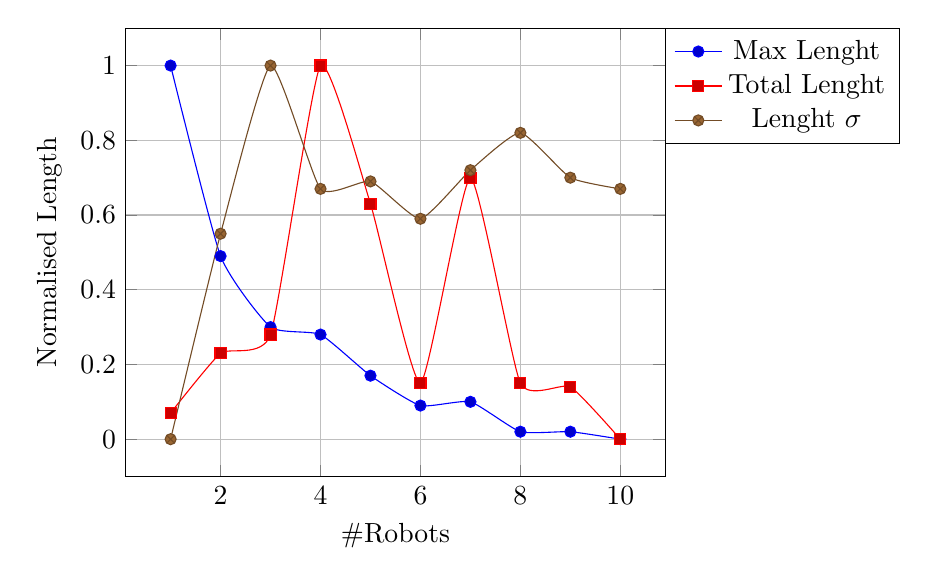
\begin{tikzpicture}
	\begin{axis}[
%		height=9cm,
%		width=9cm,
		grid=major,
                legend style = {at={(1,1)}, anchor=north west},
		xlabel=\#Robots,
		ylabel=Normalised Length,
		smooth,
		tension=0.3
	]

	\addplot coordinates {
(1, 1.00)
(2, 0.49)
(3, 0.30)
(4, 0.28)
(5, 0.17)
(6, 0.09)
(7, 0.10)
(8, 0.02)
(9, 0.02)
(10, 0.00)
	};
	\addlegendentry{Max Lenght}

	\addplot coordinates {
(1, 0.07)
(2, 0.23)
(3, 0.28)
(4, 1.00)
(5, 0.63)
(6, 0.15)
(7, 0.70)
(8, 0.15)
(9, 0.14)
(10, 0.00)
	};
	\addlegendentry{Total Lenght}

	\addplot coordinates {
(1, 0.00)
(2, 0.55)
(3, 1.00)
(4, 0.67)
(5, 0.69)
(6, 0.59)
(7, 0.72)
(8, 0.82)
(9, 0.70)
(10, 0.67)
	};
	\addlegendentry{Lenght $\sigma$}
	\end{axis}
\end{tikzpicture}
\caption{Variation of the performance indexes increasing the number of robots, for the 15x15 grid using the Node Counting algorithm}
\end{figure}


\begin{figure}[H]
\centering
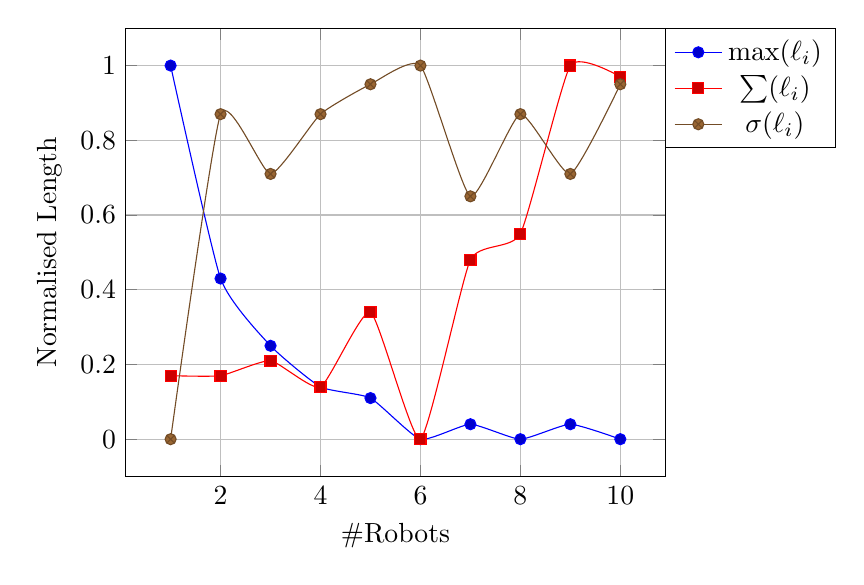
\begin{tikzpicture}
	\begin{axis}[
%		height=9cm,
%		width=9cm,
		grid=major,
                legend style = {at={(1,1)}, anchor=north west},
		xlabel=\#Robots,
		ylabel=Normalised Length,
		smooth,
		tension=0.3
	]

	\addplot coordinates {
(1, 1.00)
(2, 0.43)
(3, 0.25)
(4, 0.14)
(5, 0.11)
(6, 0.00)
(7, 0.04)
(8, 0.00)
(9, 0.04)
(10, 0.00)
	};
	\addlegendentry{$\max(\ell_i)$}

	\addplot coordinates {
(1, 0.17)
(2, 0.17)
(3, 0.21)
(4, 0.14)
(5, 0.34)
(6, 0.00)
(7, 0.48)
(8, 0.55)
(9, 1.00)
(10, 0.97)
	};
	\addlegendentry{$\sum(\ell_i)$}

	\addplot coordinates {
(1, 0.00)
(2, 0.87)
(3, 0.71)
(4, 0.87)
(5, 0.95)
(6, 1.00)
(7, 0.65)
(8, 0.87)
(9, 0.71)
(10, 0.95)
	};
	\addlegendentry{$\sigma(\ell_i)$}
	\end{axis}
\end{tikzpicture}
\caption[Perform. indexes increasing the \#robots, 5x5 grid using NC]{Performance indexes increasing the num. of robots, 5x5 grid using NC}
\end{figure}


\begin{figure}[H]
\centering
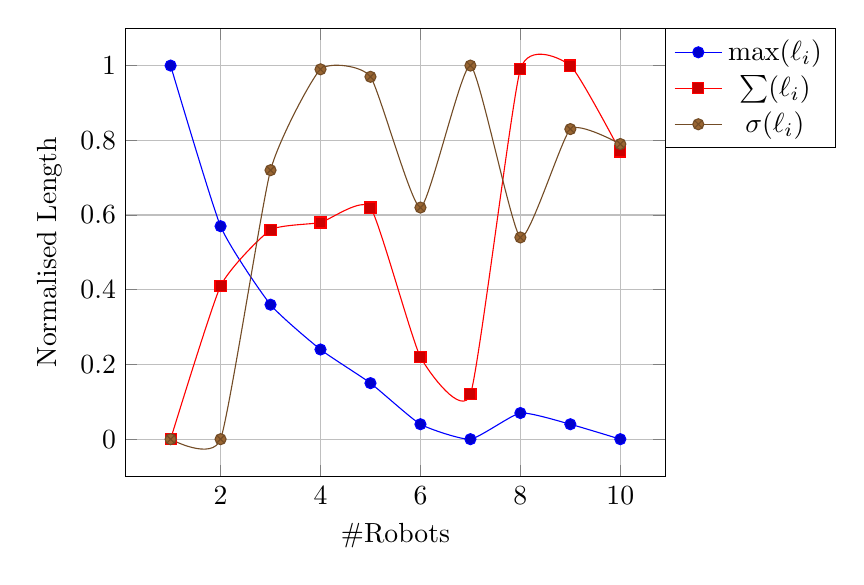
\begin{tikzpicture}
	\begin{axis}[
%		height=9cm,
%		width=9cm,
		grid=major,
                legend style = {at={(1,1)}, anchor=north west},
		xlabel=\#Robots,
		ylabel=Normalised Length,
		smooth,
		tension=0.3
	]

	\addplot coordinates {
(1, 1.00)
(2, 0.57)
(3, 0.36)
(4, 0.24)
(5, 0.15)
(6, 0.04)
(7, 0.00)
(8, 0.07)
(9, 0.04)
(10, 0.00)
	};
	\addlegendentry{$\max(\ell_i)$}

	\addplot coordinates {
(1, 0.00)
(2, 0.41)
(3, 0.56)
(4, 0.58)
(5, 0.62)
(6, 0.22)
(7, 0.12)
(8, 0.99)
(9, 1.00)
(10, 0.77)
	};
	\addlegendentry{$\sum(\ell_i)$}

	\addplot coordinates {
(1, 0.00)
(2, 0.00)
(3, 0.72)
(4, 0.99)
(5, 0.97)
(6, 0.62)
(7, 1.00)
(8, 0.54)
(9, 0.83)
(10, 0.79)
	};
	\addlegendentry{$\sigma(\ell_i)$}
	\end{axis}
\end{tikzpicture}
\caption[Perform. indexes increasing the \#robots, 10x10 grid using NC]{Performance indexes increasing the num. of robots, 10x10 grid using NC}
\end{figure}

So for the Node Counting algorithm we have that for a 5x5 map the best number of robots is 6, for the 10x10 map is 7 and for the 15x15 map is 10. The bigger leap between the last two results derives from the fact that a linear increase in the map side obviously produces a quadratic increase in the map area, thus on the size of the navigation graph. Even though no precise pattern is emerging from the relationship between number of robots and size of the map, this results give anyway an idea about the order of magnitude of the robots necessary for coverage for increasing map size.


\begin{figure}[H]
\centering
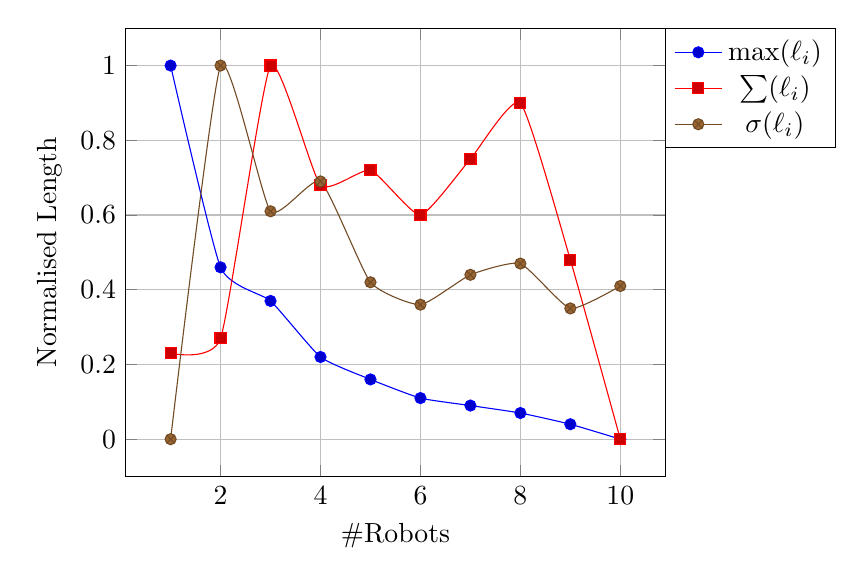
\begin{tikzpicture}
	\begin{axis}[
%		height=9cm,
%		width=9cm,
		grid=major,
                legend style = {at={(1,1)}, anchor=north west},
		xlabel=\#Robots,
		ylabel=Normalised Length,
		smooth,
		tension=0.3
	]

	\addplot coordinates {
(1, 1.00)
(2, 0.46)
(3, 0.37)
(4, 0.22)
(5, 0.16)
(6, 0.11)
(7, 0.09)
(8, 0.07)
(9, 0.04)
(10, 0.00)
	};
	\addlegendentry{$\max(\ell_i)$}

	\addplot coordinates {
(1, 0.23)
(2, 0.27)
(3, 1.00)
(4, 0.68)
(5, 0.72)
(6, 0.60)
(7, 0.75)
(8, 0.90)
(9, 0.48)
(10, 0.00)
	};
	\addlegendentry{$\sum(\ell_i)$}

	\addplot coordinates {
(1, 0.00)
(2, 1.00)
(3, 0.61)
(4, 0.69)
(5, 0.42)
(6, 0.36)
(7, 0.44)
(8, 0.47)
(9, 0.35)
(10, 0.41)

	};
	\addlegendentry{$\sigma(\ell_i)$}
	\end{axis}
\end{tikzpicture}
\caption[Perform. indexes increasing the \#robots, 15x15 grid using NC]{Performance indexes increasing the num. of robots, 15x15 grid using NC}
\end{figure}

%%%%%%%%%%%%%%%%%%%


\subsection{VRP with Floyd-Warshall}
In the following figures are plotted the results for increasing number of robots and increasing map size using the VRP Greedy coverage algorithm.

%\begin{figure}[H]
\centering
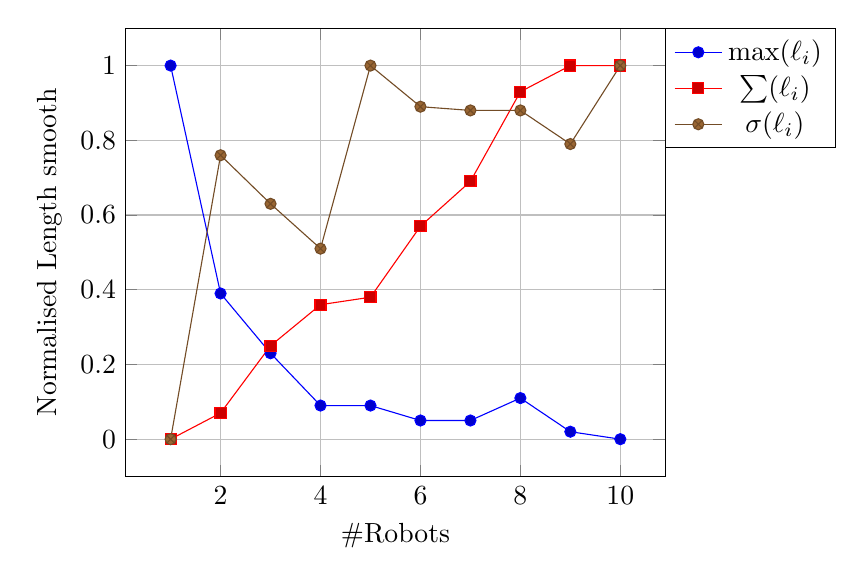
\begin{tikzpicture}
	\begin{axis}[
%		height=9cm,
%		width=9cm,
		grid=major,
                legend style = {at={(1,1)}, anchor=north west},
		xlabel=\#Robots,
		ylabel=Normalised Length
		smooth,
		tension=0.3
	]

	\addplot coordinates {
(1, 1.00)
(2, 0.39)
(3, 0.23)
(4, 0.09)
(5, 0.09)
(6, 0.05)
(7, 0.05)
(8, 0.11)
(9, 0.02)
(10, 0.00)
	};
	\addlegendentry{$\max(\ell_i)$}

	\addplot coordinates {
(1, 0.00)
(2, 0.07)
(3, 0.25)
(4, 0.36)
(5, 0.38)
(6, 0.57)
(7, 0.69)
(8, 0.93)
(9, 1.00)
(10, 1.00)
	};
	\addlegendentry{$\sum(\ell_i)$}

	\addplot coordinates {
(1, 0.00)
(2, 0.76)
(3, 0.63)
(4, 0.51)
(5, 1.00)
(6, 0.89)
(7, 0.88)
(8, 0.88)
(9, 0.79)
(10, 1.00)
	};
	\addlegendentry{$\sigma(\ell_i)$}
	\end{axis}
\end{tikzpicture}
\caption[Perform. indexes increasing the \#robots, city map using VRP]{\mbox{Performance indexes increasing the num. of robots, city map using VRP}}
\end{figure}

\begin{figure}[H]
\centering
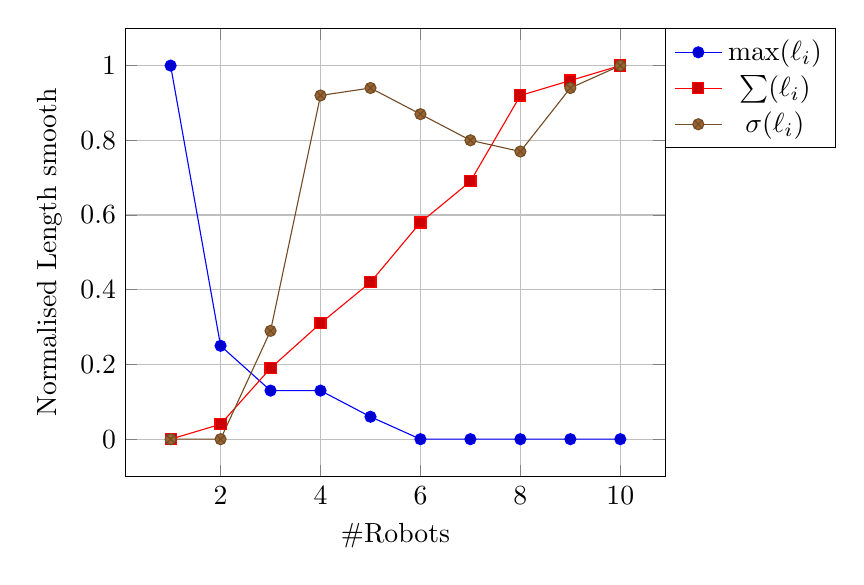
\begin{tikzpicture}
	\begin{axis}[
%		height=9cm,
%		width=9cm,
		grid=major,
                legend style = {at={(1,1)}, anchor=north west},
		xlabel=\#Robots,
		ylabel=Normalised Length
		smooth,
		tension=0.3
	]

	\addplot coordinates {
(1, 1.00)
(2, 0.25)
(3, 0.13)
(4, 0.13)
(5, 0.06)
(6, 0.00)
(7, 0.00)
(8, 0.00)
(9, 0.00)
(10, 0.00)
	};
	\addlegendentry{$\max(\ell_i)$}

	\addplot coordinates {
(1, 0.00)
(2, 0.04)
(3, 0.19)
(4, 0.31)
(5, 0.42)
(6, 0.58)
(7, 0.69)
(8, 0.92)
(9, 0.96)
(10, 1.00)
	};
	\addlegendentry{$\sum(\ell_i)$}

	\addplot coordinates {
(1, 0.00)
(2, 0.00)
(3, 0.29)
(4, 0.92)
(5, 0.94)
(6, 0.87)
(7, 0.80)
(8, 0.77)
(9, 0.94)
(10, 1.00)
	};
	\addlegendentry{$\sigma(\ell_i)$}
	\end{axis}
\end{tikzpicture}
\caption[Perform. indexes increasing the \#robots, 5x5 grid using VRP]{Performance indexes increasing the num. of robots, 5x5 grid using VRP}
\end{figure}

For the VRP algorithm we find that for a 5x5 map the best number of robots is 2, for the 10x10 map is 3 and for the 15x15 map is 5. We can clearly see how using this kind of algorithm the best number of robots is on average less than the one needed for Node Counting, that is a desirable property in term of resource saving.

\input{tex/graphs/VRP_FW_10x10_normalised}

\begin{figure}[H]
\centering
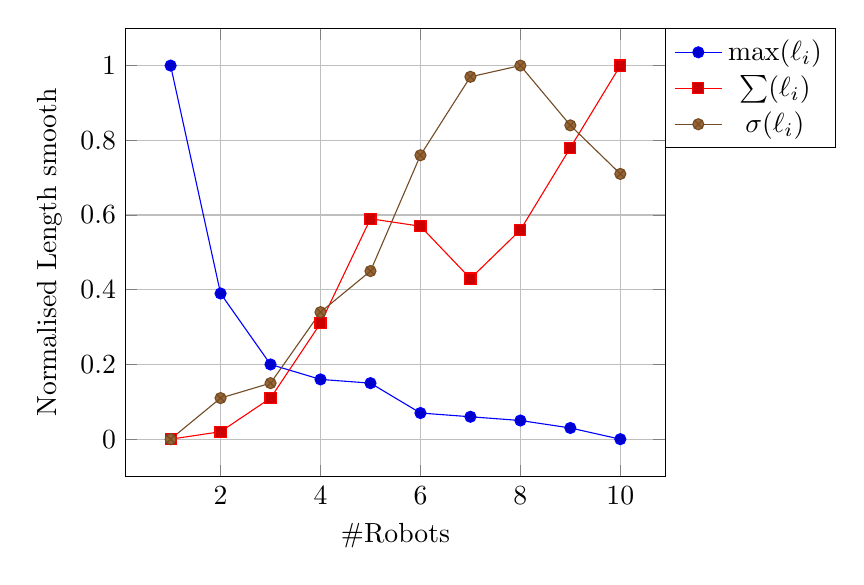
\begin{tikzpicture}
	\begin{axis}[
%		height=9cm,
%		width=9cm,
		grid=major,
                legend style = {at={(1,1)}, anchor=north west},
		xlabel=\#Robots,
		ylabel=Normalised Length
		smooth,
		tension=0.3
	]

	\addplot coordinates {
(1, 1.00)
(2, 0.39)
(3, 0.20)
(4, 0.16)
(5, 0.15)
(6, 0.07)
(7, 0.06)
(8, 0.05)
(9, 0.03)
(10, 0.00)
	};
	\addlegendentry{$\max(\ell_i)$}

	\addplot coordinates {
(1, 0.00)
(2, 0.02)
(3, 0.11)
(4, 0.31)
(5, 0.59)
(6, 0.57)
(7, 0.43)
(8, 0.56)
(9, 0.78)
(10, 1.00)
	};
	\addlegendentry{$\sum(\ell_i)$}

	\addplot coordinates {
(1, 0.00)
(2, 0.11)
(3, 0.15)
(4, 0.34)
(5, 0.45)
(6, 0.76)
(7, 0.97)
(8, 1.00)
(9, 0.84)
(10, 0.71)
	};
	\addlegendentry{$\sigma(\ell_i)$}
	\end{axis}
\end{tikzpicture}
\caption[Perform. indexes increasing the \#robots, 15x15 grid using VRP]{\mbox{Performance indexes increasing the num. of robots, 15x15 grid using NC}}
\end{figure}

In figure \ref{fig:VRPFW_execTime} is presented a comparison plot for the algorithm execution time with an increasing size of the maps.  The longest execution time has been recorded for the computation of the path for one robot in a 40 by 40 free map, for a value of $7\e{2}$ seconds, roughly 12 minutes.


\begin{figure}[H]
\centering
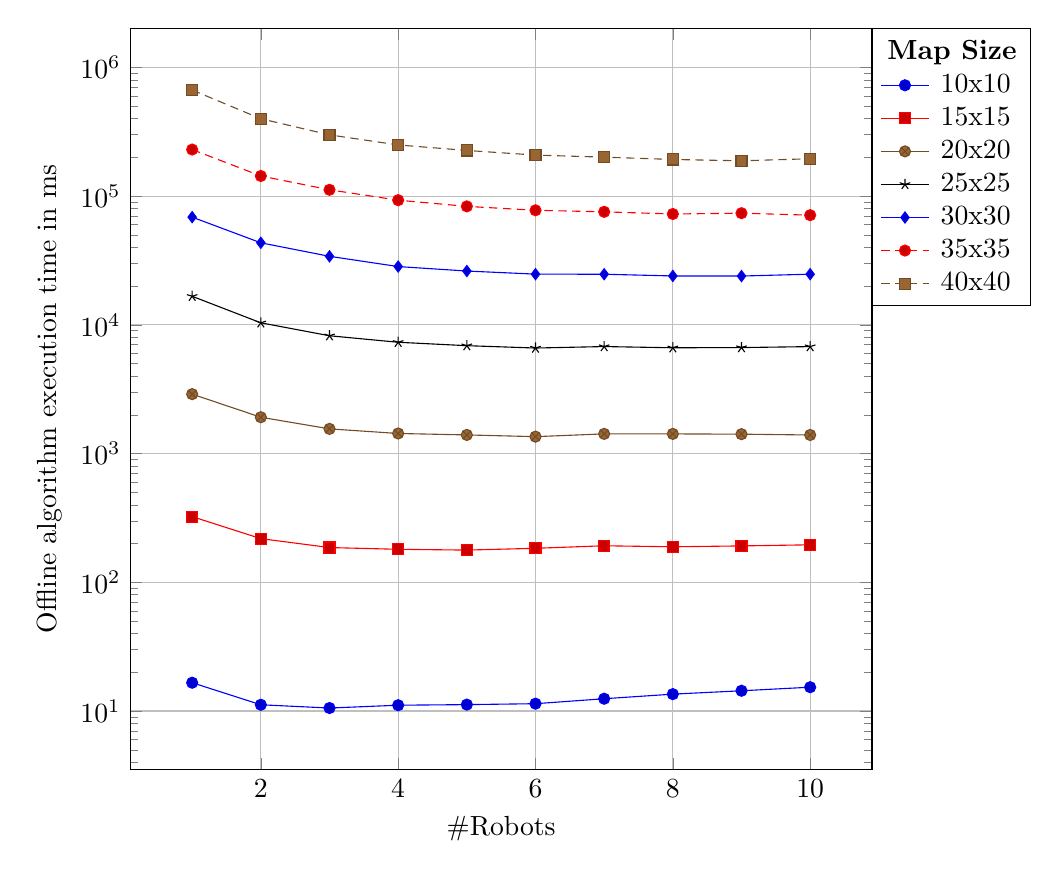
\begin{tikzpicture}
	\begin{semilogyaxis}[
		height=11cm,
		width=11cm,
                legend style = {at={(1,1)}, anchor=north west},
		grid=major,
		xlabel=\#Robots,
                   ylabel=Offline algorithm execution time in ms
	]

        \addlegendimage{empty legend}
        \addlegendentry{\hspace{-.6cm}\textbf{Map Size}}

%	\addplot coordinates {
%		(1, 0.962165)
%		(2, 0.999812)
%		(3, 3.32455)
%		(4, 1.33711)
%		(5, 1.26769)
%		(6, 4.00359)
%		(7, 4.45941)
%		(8, 1.33102)
%		(9, 1.38427)
%                (10, 3.06631)
%	};
%	\addlegendentry{5x5}

	\addplot coordinates {
		(1, 99.5812/6)
		(2, 67.1215/6)
		(3, 63.3223/6)
		(4, 66.5972/6)
		(5, 67.303/6)
		(6, 68.4257/6)
		(7, 74.7808/6)
		(8, 81.1845/6)
		(9, 86.226/6)
                (10, 91.9106/6)
	};
	\addlegendentry{10x10}

	\addplot coordinates {
		(1, 1941.57/6)
		(2, 1310.12/6)
		(3, 1117.07/6)
		(4, 1082.52/6)
		(5, 1067.53/6)
		(6, 1102.4/6)
		(7, 1153.16/6)
		(8, 1132.38/6)
		(9, 1150.22/6)
                (10, 1173.2/6)
	};
	\addlegendentry{15x15}

	\addplot coordinates {
		(1, 17361.1/6)
		(2, 11490/6)
		(3, 9328.54/6)
		(4, 8591.75/6)
		(5, 8372.56/6)
		(6, 8116.5/6)
		(7, 8529.95/6)
		(8, 8526.77/6)
		(9, 8485.28/6)
                (10, 8361.64/6)
	};
	\addlegendentry{20x20}

	\addplot coordinates {
		(1, 99929.9/6)
		(2, 62180.2/6)
		(3, 49326.2/6)
		(4, 43910.5/6)
		(5, 41311.1/6)
		(6, 39607.3/6)
		(7, 40667/6)
		(8, 39792/6)
		(9, 39942.7/6)
                (10,40629.5/6)
	};
	\addlegendentry{25x25}

	\addplot coordinates {
		(1, 411589/6)
		(2, 260044/6)
		(3, 204265/6)
		(4, 170023/6)
		(5, 156969/6)
		(6, 148516/6)
		(7, 148225/6)
		(8, 143764/6)
		(9, 143510/6)
                (10, 148387/6)
	};
	\addlegendentry{30x30}

	\addplot coordinates {
		(1, 1.37889e+06/6)
		(2, 859312/6)
		(3, 671124/6)
		(4, 557420/6)
		(5, 498969/6)
		(6, 465257/6)
		(7, 452598/6)
		(8, 435339/6)
		(9, 441815/6)
                (10, 426400/6)
	};
	\addlegendentry{35x35}

	\addplot coordinates {
		(1, 3.99748e+06/6)
		(2, 2.39203e+06/6)
		(3, 1.79249e+06/6)
		(4, 1.49702e+06/6)
		(5, 1.35637e+06/6)
		(6, 1.24861e+06/6)
		(7, 1.20327e+06/6)
		(8, 1.15456e+06/6)
		(9, 1.12716e+06/6)
                (10, 1.16961e+06/6)
	};
	\addlegendentry{40x40}
	
	\end{semilogyaxis}
\end{tikzpicture}
\caption{VRP-FloydWarshall:  Different execution times for growing map sizes}
\label{fig:VRPFW_execTime}
\end{figure}








\pagebreak


\section{Conclusions}
We have seen how for the multi-robot coverage problem the elementary Node Counting algorithm resulted to be one of the most efficient solutions, with final paths lengths even comparable with the VRP Greedy ones. The most interesting results being the one of the ``vertex oriented'' algorithms Node Counting and LRTA*, the latter suffering for the intrinsic inefficient mechanism implemented for the update rule in the multi-robot case (section \ref{sec:LRTAstar}). ``Edge oriented'' algorithm as Edge Counting and PatrolGRAPH* do not seem to fit the needs of the coverage problem as they always end up in longer paths with respected to the vertex oriented algorithms.
The VRP algorithm seems anyway to achieve the overall best results in very large obstacle-free maps, which can be the case for high altitude flight. An undeniable advantage of the VRP algorithm also is that the solution is almost instant giving us an idea of the total coverage time, a very useful information in SAR applications.



\chapter{Experiments With Real Multi-copters}

As a final step the algorithms were tested using two high-end quadcopters available in the laboratory. In particular the multi-copters are produced by Ascending Technologies and are:
\begin{itemize}
\item Asctec Firefly (hexacopter)
\item Asctec Pelican (quadcopter)
\end{itemize}

\begin{figure}[H] 
  \begin{minipage}[b]{0.5\linewidth}
    \centering
    \includegraphics[width=0.8\textwidth]{asctec_firefly}
    \caption{Asctec Firefly}
    \label{fig:firefly}
    \vspace{4ex}
  \end{minipage}
  \begin{minipage}[b]{0.5\linewidth}
    \centering
    \includegraphics[width=0.7\textwidth]{asctec_pelican}
    \caption{Asctec Pelican}
    \label{fig:pelican}
    \vspace{4ex}%%
  \end{minipage}
\end{figure}


They both mount an on-board computer which runs Linux and Wi-Fi adapter through which is performed all the communication. For the robot dynamic control system is used the ETHNOS \cite{ethnos2000} real-time software framework. The ETHNOS environment is composed of a dedicated distributed real-time operating system (developed as an extension to Linux), with a dedicated network protocol designed for both the single robot and the multi-robot environment, specifically designed for noisy wireless communication. The waypoint controller, from the algorithm to the robot CU, is implemented using a dedicated ROS/ETHNOS interface the communication between the path planner and.


\section{Multi-rotor model and parameters tuning}


During the experiments ``on the field'' the main part was spent in the fine tuning of the quadcopters controllers. In particular by adjusting the PID parameters that control the propellers thrust in reaching a given target. In this section we will give a general idea of the control scheme and how this applies to the quadcopter dynamics.

To describe the ideal dynamics of a multi-rotor aircraft we can use the following mathematical model \cite{2010JSDD4255A}:

\begin{equation}
  \begin{cases}
   \ddot{\xi} = \frac{1}{m}uR{e_3}-g{e_3} \\
   M(\eta)\ddot{\eta}+C(\eta,\dot{\eta})\dot{\eta} = \Uppsi(\eta)^{T}\tau
  \end{cases}
\end{equation}

where $m,\xi$ and $\eta$ are the aircraft mass, position and orientation respectively. $(u, \tau)$ are the applied thrust and torque vector, $R$ and $\Uppsi$ are the rotation matrix and Euler matrix respectively. \\% The pseudo inertial matrix $M$ is defined as $M(\eta) = \Uppsi(\eta)^{T}J\Uppsi(\eta)$, and the centripetal vector C is given by \mbox{$C(\eta,\dot{\eta}) =  \Uppsi(\eta)^{T}J\dot{\Uppsi}(\eta)-\Uppsi(\eta)^{T}sk(\Uppsi(\eta)\dot{\eta})J\Uppsi(\eta)$}.
For autonomous multi-rotors it is common to separate the flight control problem into an ``inner-loop'' that controls attitude and an ``outer-loop'' that controls the translational trajectory of the aircraft. After transforming the original system into one that describes the position dynamics \cite{kendoul:hal-00338358} we can finally the PID controller as follows:

\begin{equation}
\mu{_x} = - K_{P_x}(x - x_d) - K_{I_x} \int (x - x_d) dt - K_{D_x}(v_x-v_{x}d)
\end{equation}

And the same goes for $y$ and $z$. This is the so called outer-loop position control. $\mu$ is an intermediate control vector and after evaluating $\mu{_x}$, $\mu{_y}$ and $\mu{_z}$ we can calculate the desired thrust $u$, roll angle $\phi_d$ and pitch angle $\theta_d$ that  constitutes the input parameters for the inner-loop , the \emph{attitude controller}:

\begin{equation}
  \begin{cases}
   u = m \sqrt{{\mu{_x}}^2 + {\mu{_y}}^2 + {(\mu{_z}+g)}^2} \\
  \phi_d = sin^{-1} \left( m\dfrac{ \mu{_x} sin\psi_d - \mu{_y} cos\psi_d }{ u } \right) \\
  \theta_d = tan^{-1} \left( \dfrac{ \mu{_x} cos\psi_d - \mu{_y} sin\psi_d }{ \mu{_x} + g} \right)
  \end{cases}
\end{equation}

where $g$ is the gravity acceleration that has to be compensated to fly and $\psi_d$ is the yaw angle which represent the aircraft heading direction. In general $\psi_d$ can be set to zero, as the orientation of the multi-rotor is not relevant unless it mounts some front directional camera. The attitude controller will then care of transforming these values into input controls for the aircraft's propellers. The standard PID controller can be represented using a block diagram as in Fig. \ref{fig:pid_blockDiag}.

\begin{figure}[h]
\includegraphics[width=\textwidth]{pid_controller}
\caption{A general PID controller block diagram}
\label{fig:pid_blockDiag}
\end{figure}


To have any kind of control over the quadcopter or multi-copter, we need to be able to measure the quadcopter sensor output (for example the pitch angle), so we can estimate the error (how far we are from the the desired pitch angle, e.g. horizontal, 0 degree). We can then apply the three proportional (P), integrative (I) and derivative (D) control algorithms to the error, to get the next outputs for the motors aiming to correct the error.

The three parameters that we can adjust to improve better quadcopter stability are the $K_P$, $K_I$, $K_D$ gains showed in Fig. \ref{fig:pid_blockDiag}. Each gain coefficent basically would change the importance and influence of each algorithm to the output. Let's now look at what are the effects of these parameters to the stability of a quadcopter.


Since we want to control the quadcopter's $(x,y,z)$ position in space, the parameters will be described in terms of how they affect the process of keeping the desired position.

The proportional gain coefficient $K_P$ determines how fast the quadcopter will reach the desired position. The higher the coefficient, the higher the multi-copter will be sensitive and reactive to position change. If it is too low, the quadcopter will appear sluggish and will be harder to keep steady. If the P gain is too high the multi-copter may start to oscillate with a high frequency and overshoot the target repeatedly. %
The integral gain coefficient $K_I$ can increase the precision of the final position since it will eliminate the so called \emph{steady-state error}. This term is especially useful with irregular wind, and ground effect (turbulence from motors). However, when the $K_I$ value gets too high your quadcopter might begin to have slow reaction and a decrease effect of the proportional gain as consequence, it will also start to oscillate like having high $K_P$ gain, but with a lower frequency. %
The derivative gain coefficient $K_D$ will impact what the other two gain cannot control that is reduce the overshoot and the settling time. It will also work like a damping factor against the previous two, to prevent excessive oscillation in a situation of high $K_P$ and $K_I$. It  This parameter is extremely delicate since it depends on the rate of change of the error and in certain cases it may amplify the effects of the previous gains.  %

Since finding the exact parameters of the mathematical model of each quadcopter can be extremely difficult the most common way to tune this parameters is by trial and error. In the following paragraph there are a couple rules of thumb. To tune quadcopter $K_P$ gain the procedure is to slowly increase it until the quadcopter reaches the position without producing big oscillations. For the $K_I$ gain, again start low and increase slowly, paying attention to how long does it take to stop and stabilize. You want to get to a point where it stabilize very quickly while not wandering around for too long. To get a reliable I-value a test under windy condition may be useful. For $K_D$ gain, it can get into a complicated interaction with $K_P$ and $K_I$ values. When using D gain, you need to go back and fine tune P and I to keep the plant well stabilized.

\section{Results}

Here we present the results for the Node Counting algorithm using the the two aircraft. Since the test were performed just to check that everything was working properly, the map used is a very simple 3x3 grid map, where every cell has a side of 5m.

\begin{figure}[H] 
  \begin{minipage}[b]{0.5\linewidth}
    \centering
    \includegraphics[width=0.9\textwidth]{fir_x170800_y170800_z1700800_b}
    \caption{Firefly path, $\ell$=8}
    \label{fig:pel_path}
    %\vspace{4ex}
  \end{minipage}
  \begin{minipage}[b]{0.5\linewidth}
    \centering
    \includegraphics[width=0.9\textwidth]{pel_x200800_y200800_z3001200_b}
    \caption{Pelican path, $\ell$=12}
    \label{fig:fir_path}
   % \vspace{4ex}
  \end{minipage}
\end{figure}

In the figures \ref{fig:pel_path} and \ref{fig:fir_path} we can see two separate runs of the coverage. The green polygonal chain is used as a reference and is an ideal, yet unfeasible, path of the coverage. The blue curve instead is path followed by the real aircraft and we can see that in both cases we have a very good behaviour on the x-y plane.
In the next two figures instead we have the resulting paths for a double-robot coverage, in red the Asctec Firefly while in blue the Asctec Pelican. \\

%Quadcopters paths:
%#0: 0 1 2 5 8
%#1: 0 3 4 7 6

%Quadcopters paths:
%#0: 0 1 2 1 4 
%#1: 0 3 4 5 8 7 6

\begin{figure}[H]
  \begin{minipage}[b]{0.5\linewidth}
    \centering
    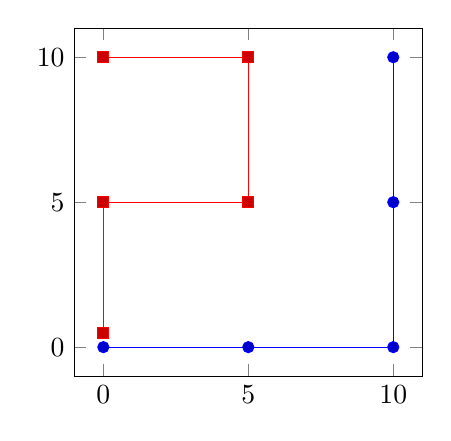
\begin{tikzpicture}
	\begin{axis}[
		height=6cm,
		width=6cm
	       ]

	\addplot coordinates {
(0, 0)
(5, 0)
(10, 0)
(10, 5)
(10, 10)
	};
	\addplot coordinates {
(0, 0.5)
(0, 5)
(5, 5)
(5, 10)
(0, 10)
	};
	\end{axis}
\end{tikzpicture}
    \caption{Coverage (a)}
    \label{fig:asctec_double_a}
    %\vspace{4ex}
  \end{minipage}
  \begin{minipage}[b]{0.5\linewidth}
    \centering
        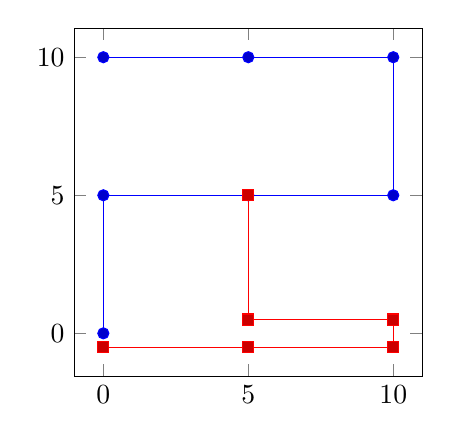
\begin{tikzpicture}
	\begin{axis}[
		height=6cm,
		width=6cm
		]

	\addplot coordinates {
(0, 0)
(0, 5)
(5, 5)
(10, 5)
(10, 10)
(5, 10)
(0, 10)
	};
	\addplot coordinates {
(0, -0.5)
(5, -0.5)
(10, -0.5)
(10, 0.5)
(5, 0.5)
(5, 5)
	};
	\end{axis}
\end{tikzpicture}
    \caption{Coverage (b)}
    \label{fig:asctec_double_b}
   % \vspace{4ex}
  \end{minipage}
\end{figure}


\noindent In the coverage (b), Fig. \ref{fig:asctec_double_b}, we can see that the firefly was slower than the pelican so the former found an already visited node in $(10,5)$ causing it to retrace his steps.

On the whole the results show that the framework has proved to be fully functional. The most important aspect is that due to the approach used in creating the coverage logic, the code is implemented to be easily scalable and ready to be applied on a bigger number of multi-copters.

\chapter{Additional details}


\section{About the code}

In this section a couple of technicalites are described for who is interested in deepening the knowledge of the software implementation. There is somehow a logic beyond the name of the source files: all the files that start with the \emph{quad} prefix are controlling the quadcopters in the simulator via ROS and are consequently executable files. To plan the paths the executables  make use of libraries implemented in the relative classes. For example the node counting algorithm is implemented in the \texttt{NodeCounting.cpp} class, used by  \texttt{quadNodeCount.cpp} to control the movements of the quadcopters in the simulator.
All the code was finally compiled with the gcc optimization level ``-O3'' enabled, by setting in the \texttt{CMakeList.txt} the \emph{release} build type.
The code is designed to be fairly flexible making large use of input arguments in order easily run the simulation using different parameters without having to recompile the code each time. The input parameters for the online and offline algorithms (\texttt{quad*.cpp} files) are slightly different due do the different nature of the two, and are listed in table \ref{tab:inputArgs}.

\begin{table}[h]
\centering
\begin{tabular}{@{}cccc@{}}
\toprule
\textbf{argv{[}$\cdot${]}} & \multicolumn{3}{c}{\textbf{Corresponding Parameter}}                                                                   \\ \cmidrule(l){2-4} 
            & Online robot controller    & Offline robot controller      & Offline kernelNode        \\ \midrule
1           & Robot ID\#                   &   Robot ID\#                     & Input map          \\
2           & Input map                    & Height of flight (z)             & \# of robots         \\
3           & Height of flight (z)         & Control Mode                    &                           \\
4           & Control Mode                &                                       &                           \\
5           & Starting vertex              &                                        &                           \\
6           & Min visits per vertex      &                                        &                           \\ \bottomrule
\end{tabular}
\caption{Input arguments for the coverage algorithms}
\label{tab:inputArgs}
\end{table}


As we can see in the offline case the parameters are spread between the controller and the kernelNode that generate the paths. The \emph{Control Mode} argument is used to change the waypoint planning algorithm for switching between the simulator and the real multi-copters control.

\section{Open Licensing}

\begin{aquote}{L. Torvalds}
``In open source, we feel strongly that to really do something well, you have to get a lot of people involved.''
\end{aquote}

Following the attitude which inspired Torvalds, and the \emph{not reinventing the wheel} paradigm, all the code developed in this thesis is released with open source licenses such as MIT License and BSD License. Mixing this two licenses is possible since they are both ``GPL-compatible''. For more info visit \href{http://opensource.org/licenses}{OSI: Licenses} and \href{http://en.wikipedia.org/wiki/License_compatibility}{License Compatibility}. The source files can be found on GitHub in the \href{https://github.com/merosss/VRepRosQuadSwarm}{VRepRosQuadSwarm} repository.

The same attitude has been followed for the software tools used: Ubuntu, ROS, Coppelia Robotics VREP Simulator and LibreOffice are all open source projects. The 3D models used to create the simulation environment are free models, downloaded at \href{http://tf3dm.com/}{TF3DM}. As you probably have already noticed this thesis is written in \LaTeX, also distributed under a free software license.


\begin{appendices}
\chapter{First iterations of the online coverage algorithms}
\label{app:firstSteps}

To observe the behaviour of the algorithms we will look at the evolution of the \emph{Count Map}, that is the matrix that contains the visits count for all the vertices in the graph. The map used for this purposes is 4x4 obstacle free grid-map. For simplicity let's imagine to sample the time every time we reach a new vertex (a cell of the map). To be able to look at a fairly wide time window, for all the algorithms are presented the count maps for $t$=0, $t$=3, $t$=6, $t$=9.

In the pictures we will consider the time instant when the robot has just arrived on the current cell but not yet made is decision on the next move. The cell in which the robot is currently on is highlighted in grey.

\captionsetup[table]{name=Fig.}

%%%%%%%%%%%%%%

\section{Node Counting}


\begin{table}[H]
    \begin{minipage}{.24\linewidth}
      \centering
       \taburulecolor{lightgray}
       \addtocontents{lot}{\SkipTolEntry}
       \begin{tabu}{|c|c|c|c|}
       \hline
         \cellcolor{lightgray}1 & 0 & 0 & 0 \\ \hline
         0 & 0 & 0 & 0 \\ \hline
         0 & 0 & 0 & 0 \\ \hline
         0 & 0 & 0 & 0 \\ \hline
        \end{tabu}
       \caption{$t$=0}
      \end{minipage}
     %\quad%%%%%%%
   \begin{minipage}{.24\linewidth}
      \centering
       \taburulecolor{lightgray}
       \addtocontents{lot}{\SkipTolEntry}
       \begin{tabu}{|c|c|c|c|}
       \hline
         1 & 1 & 1 & 0 \\ \hline
         0 & 0 &\cellcolor{lightgray}1 & 0 \\ \hline
         0 & 0 & 0 & 0 \\ \hline
         0 & 0 & 0 & 0 \\ \hline
        \end{tabu}
       \caption{$t$=3}
      \end{minipage}
   %  \quad%%%%%%%
   \begin{minipage}{.24\linewidth}
      \centering
       \taburulecolor{lightgray}
       \addtocontents{lot}{\SkipTolEntry}
       \begin{tabu}{|c|c|c|c|}
       \hline
         1 & 1 & 1 & 0 \\ \hline
         0 & 0 & 1 & 0 \\ \hline
         \cellcolor{lightgray}1 & 1 & 1 & 0 \\ \hline
         0 & 0 & 0 & 0 \\ \hline
        \end{tabu}
       \caption{$t$=6}
      \end{minipage}
    % \quad%%%%%%%
   \begin{minipage}{.24\linewidth}
      \centering
       \taburulecolor{lightgray}
       \addtocontents{lot}{\SkipTolEntry}
       \begin{tabu}{|c|c|c|c|}
       \hline
         1 & 1 & 1 & 0 \\ \hline
         0 & 0 & 1 & 0 \\ \hline
         1 & 1 & 1 & 0 \\ \hline
         1 & 1 & \cellcolor{lightgray}1 & 0 \\ \hline
        \end{tabu}
       \caption{$t$=9}
      \end{minipage}
\caption{Node Counting visit count map}
\end{table}


\clearpage
%%%%%%%%%%%%%%

\section{Learning Real-Time A*}
For the Learning Real Time A* in addition to the visits count map is presented the \emph{LRTA-count} one, following the LRTA update rule as in algorithm \ref{alg:rt_lrta}.

\input{./tex/tables/LRTA_firstSteps}


\begin{table}[H]
    \begin{minipage}{.24\linewidth}
      \centering
       \taburulecolor{lightgray}
       \addtocontents{lot}{\SkipTolEntry}
       \begin{tabu}{|c|c|c|c|}
       \hline
         \cellcolor{lightgray}0 & 0 & 0 & 0 \\ \hline
         0 & 0 & 0 & 0 \\ \hline
         0 & 0 & 0 & 0 \\ \hline
         0 & 0 & 0 & 0 \\ \hline
        \end{tabu}
       \caption{$t$=0}
      \end{minipage}
     %\quad%%%%%%%
   \begin{minipage}{.24\linewidth}
      \centering
       \taburulecolor{lightgray}
       \addtocontents{lot}{\SkipTolEntry}
       \begin{tabu}{|c|c|c|c|}
       \hline
         1 & 1 & 1 & 0 \\ \hline
         0 & 0 & \cellcolor{lightgray}0 & 0 \\ \hline
         0 & 0 & 0 & 0 \\ \hline
         0 & 0 & 0 & 0 \\ \hline
        \end{tabu}
       \caption{$t$=3}
      \end{minipage}
   %  \quad%%%%%%%
   \begin{minipage}{.24\linewidth}
      \centering
       \taburulecolor{lightgray}
       \addtocontents{lot}{\SkipTolEntry}
       \begin{tabu}{|c|c|c|c|}
       \hline
         1 & 1 & 1 & 2 \\ \hline
         0 & 0 & 1 & \cellcolor{lightgray}1 \\ \hline
         0 & 0 & 0 & 0 \\ \hline
         0 & 0 & 0 & 0 \\ \hline
        \end{tabu}
       \caption{$t$=6}
      \end{minipage}
    % \quad%%%%%%%
   \begin{minipage}{.24\linewidth}
      \centering
       \taburulecolor{lightgray}
       \addtocontents{lot}{\SkipTolEntry}
       \begin{tabu}{|c|c|c|c|}
       \hline
         1 & 1 & 1 & 2 \\ \hline
         0 & 0 & 1 & 1 \\ \hline
         0 & 0 & 0 & 1 \\ \hline
         0 & 0 & \cellcolor{lightgray}0 & 1 \\ \hline
        \end{tabu}
       \caption{$t$=9}
      \end{minipage}
\caption{LRTA-count map}
\end{table}


%%%%%%%%%%%%%%

\section{Edge Counting}

\input{./tex/tables/EC_firstSteps}

%%%%%%%%%%%%%%

\section{PatrolGRAPH*}

\input{./tex/tables/PG_firstSteps}












\end{appendices}


\singlespace
\bibliographystyle{plain} % Arrange the bibliography in order of appearance
\bibliography{MasterThesis}


\end{document}

%   VARIOUS SNIPPETS OF CODE:

%\[
%\left|\sum_{i=1}^n a_ib_i\right|
%\le
%\left(\sum_{i=1}^n a_i^2\right)^{1/2}
%\left(\sum_{i=1}^n b_i^2\right)^{1/2}
%\]
